%\documentclass[sigchi, review]{acmart}
\PassOptionsToPackage{table}{xcolor}
\documentclass[sigchi]{acmart}
\settopmatter{printacmref=false} % Removes citation information below abstract
\renewcommand\footnotetextcopyrightpermission[1]{} % removes footnote with conference information in first column
\pagestyle{plain} % removes running headers
% Load basic packages
\usepackage{balance}  % to better equalize the last page
\usepackage{graphics} % for EPS, load graphicx instead
\usepackage[T1]{fontenc}
\usepackage{txfonts}
\usepackage{mathptmx}
\usepackage[htt]{hyphenat}
% \usepackage[pdftex]{hyperref}

% \usepackage{booktabs}
% \usepackage{textcomp}
\usepackage{xspace}
\usepackage{setspace}
\usepackage{graphicx}
\usepackage{caption}
\usepackage[textsize=tiny]{todonotes}
% Some optional stuff you might like/need.
\usepackage{microtype} % Improved Tracking and Kerning
% \usepackage[all]{hypcap}  % Fixes bug in hyperref caption linking
\usepackage{ccicons}  % Cite your images correctly!
% \usepackage[utf8]{inputenc} % for a UTF8 editor only
\usepackage{verbatim}
\usepackage{relsize}
\usepackage{etoolbox}
\usepackage{lipsum}   % for filler text
\usepackage{setspace} % for \onehalfspacing and \singlespacing macros
\usepackage[normalem]{ulem}
\usepackage{enumitem}
\usepackage{relsize,etoolbox}% http://ctan.org/pkg/{relsize,etoolbox}
\usepackage{makecell}
\renewcommand\theadalign{bc}
\renewcommand\theadgape{\Gape[4pt]}
\renewcommand\cellgape{\Gape[4pt]}
\AtBeginEnvironment{quote}{\small}% Step font down one size relative to current font.
\setcopyright{none}

% DOI
\acmDOI{10.475/123_4}

% ISBN
\acmISBN{123-4567-24-567/08/06}

%Conference
\acmConference[CHI]{ACM CHI}{2019}{}
\acmYear{2019}
\copyrightyear{2019}

\acmPrice{15.00}

\def\plaintitle{Accelerating Scientific Data Exploration \\ via Visual Query Systems}
\def\emptyauthor{}
\def\plainkeywords{Data visualization, exploratory data analysis, visual query, scientific data.}
\def\plaingeneralterms{Documentation, Standardization}

% llt: Define a global style for URLs, rather that the default one
\makeatletter
\def\url@leostyle{%
  \@ifundefined{selectfont}{
    \def\UrlFont{\sf}
  }{
    \def\UrlFont{\small\bf\ttfamily}
  }}
\makeatother

\newenvironment{denselist}{
    \begin{list}{\small{$\bullet$}}%
    {\setlength{\itemsep}{0ex} \setlength{\topsep}{0ex}
    \setlength{\parsep}{0pt} \setlength{\itemindent}{0pt}
    \setlength{\leftmargin}{1.5em}
    \setlength{\partopsep}{0pt}}}%
    {\end{list}}

\newcommand{\squishlist}{
   \begin{list}{$\bullet$}
    { \setlength{\itemsep}{0pt}
      \setlength{\parsep}{2pt}
      \setlength{\topsep}{0pt}
      \setlength{\partopsep}{0pt}
      \leftmargin=25pt
\rightmargin=0pt
\labelsep=5pt
\labelwidth=10pt
\itemindent=0pt
\listparindent=0pt
\itemsep=\parsep
    }
}
\newcommand*{\img}[1]{%
    \raisebox{-.3\baselineskip}{%
        \includegraphics[
        height=\baselineskip,
        width=\baselineskip,
        keepaspectratio,
        ]{#1}%
    }%
}
\newcommand{\squishend}{\end{list}}
\newcommand{\npar}{\par\noindent}
% use extensively to toggle between paper and TR
\newcommand{\eat}[1]{}
% \newcommand{\papertext}[1]{{\leavevmode\color{blue}{#1}}}
% \newcommand{\techreport}[1]{{\leavevmode\color{red}{#1}}}
\newcommand{\papertext}[1]{#1}
\newcommand{\techreport}[1]{}
\newcommand{\nonannon}[1]{#1}
\newcommand{\annon}[1]{}
\newcommand{\boldpara}[1]{\par\noindent\textbf{#1}}
% de-facto paragraph format
\newcommand{\stitle}[1]{\noindent\textbf{#1}}
\newcommand{\tvcg}[1]{#1}
\newcommand{\cut}[1]{{\leavevmode\color{lightgray}{#1}}}
\newcommand{\ccut}[1]{} %confirmed cut

\urlstyle{leo}

% To make various LaTeX processors do the right thing with page size.
\def\pprw{8.5in}
\def\pprh{11in}
\special{papersize=\pprw,\pprh}
\setlength{\paperwidth}{\pprw}
\setlength{\paperheight}{\pprh}
\setlength{\pdfpagewidth}{\pprw}
\setlength{\pdfpageheight}{\pprh}

% create a shortcut to typeset table headings
% \newcommand\tabhead[1]{\small\textbf{#1}}
\newcommand{\zv}{\textit{zenvisage}\xspace}
\newcommand{\astro}{\textit{astro}\xspace}
\newcommand{\bio}{\textit{genetics}\xspace}
\newcommand{\matsci}{\textit{matsci}\xspace}

\newcommand{\agp}[1]{\textcolor{teal}{Aditya: #1}}
\newcommand{\kk}[1]{\textcolor{red}{Karrie: #1}}
\newcommand{\dor}[1]{\textcolor{violet}{Doris: #1}}


%%%%%%%%%%%%%%%%%%%%%%%%%%%%%%%%%%%%%%%%%%%%%%%%%%%%%%%%%%%%%%%%
%%%%%%%%%%%%%%%%%%%%%% START OF THE PAPER %%%%%%%%%%%%%%%%%%%%%%
%%%%%%%%%%%%%%%%%%%%%%%%%%%%%%%%%%%%%%%%%%%%%%%%%%%%%%%%%%%%%%%%%

\begin{document}
% \title{Understanding usage patterns for query specification in sketch-based visual query systems: A Case Study with Zenvisage}
\title{How are visual query systems used in practice: A Design Study with Zenvisage}

\begin{abstract}
The increasing availability of rich and complex data in a variety of scientific domains poses a pressing need for tools to enable scientists to rapidly make sense of and gather insights from data. One proposed solution is to design visual query systems (VQSs) that allow scientists to interactively search for desired patterns in their datasets. While many existing VQSs promise to accelerate exploratory data analysis by facilitating this search, they are not widely used in practice. Through a year-long collaboration with scientists in three distinct domains---astronomy, genetics, and material science---we study the impact of various features within VQSs that can aid rapid visual data analysis, and how VQSs fit into scientists' analysis workflow. Our findings offer design guidelines for improving the usability and adoption of next-generation VQSs, paving the way for VQSs to be applied to a variety of scientific domains.
\end{abstract}
\keywords{Visual analytics, visualization, exploratory data analysis, visual query, scientific data.}
% Note that keywords are not normally used for peerreview papers.
% \begin{teaserfigure}
% % \begin{figure}[h!]
%     \centering
%     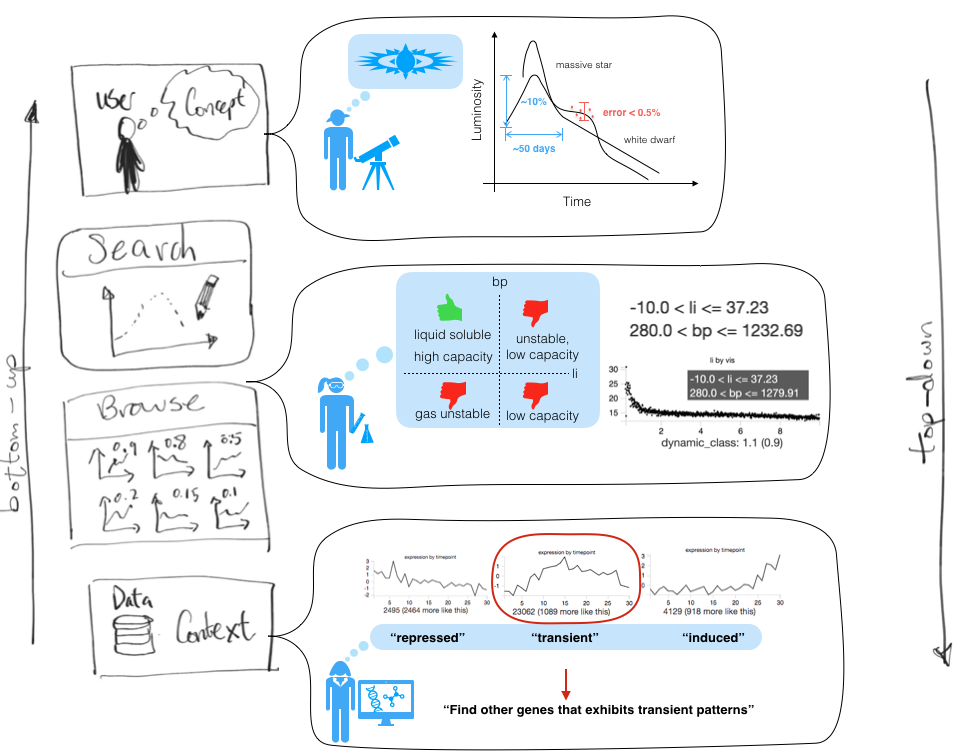
\includegraphics[width=0.6\linewidth]{figures/search-browse-model.png}
%     \vspace{-6pt}\caption{Search Browse Model}
%     \label{sbmodel}
%     \vspace{-5pt}
% % \end{figure}
% \end{teaserfigure}
\maketitle

%!TEX root=main.tex
\vspace{-5pt}
\section{Introduction\label{sec:intro}}
% one for each key finding: a) many features deemed to be of importance to VQSs by domain experts, not all supported by present-day VQSs b) sketch is inefficient, perhaps explaining why present-day VQSs are not popular c) identify 3 typical workflows involving various sensemaking modalities in different proportions, depending on the application
Line charts are commonly employed during data exploration---the
intuitive connected patterns
often illustrate complex underlying processes
and yield interpretable and visually compelling data-driven
narratives.
To discover patterns in line charts,
analysts construct them
using toolkits like \texttt{ggplot} or \texttt{matplotlib},
or visualization construction interfaces
like Excel or Tableau, specifying
{\em exactly} what they want to visualize.
For example, when trying to find celestial objects
corresponding to supernovae, which have a specific pattern
of brightness over time, astronomers
individually inspect the corresponding line chart
for each object (often numbering in the hundreds)
until they find ones that match the pattern. \ccut{Similarly, when trying to infer relationships between two physical properties for different subsets of battery electrolytes, scientists need to individually visualize these properties
for each subset (out of an unbounded number of such subsets)
until they identify relationships that make sense to them.}
This process of manual exploration of
large numbers of line charts
is not only error-prone, but also overwhelming for
analysts.
%, not only for time series but also for understanding the relationships between multiple measures variables.

% From high-throughput genome sequencing,
% to multi-resolution astronomical imaging telescopes,
% to at-scale physical testing of battery candidates,
% many fields of science and engineering
% are facing an increasing availability of
% large volumes of complex data~\cite{AustinNothaft2015,Demchenko2013},
% holding the key to some of the most pressing
% unanswered scientific questions of our time,
% such as: How does a treatment affect the
% expression of a gene in a breast cancer cell-line?
% Which battery components have sustainable levels
% of energy-efficiency and are safe and cheap to
% manufacture in production?
% While data analysis is central to a scientist's
% knowledge discovery process, scientists
% often lack the extensive experience to deal
% with data of this scale and complexity
% in a way that can facilitate rapid insight discovery~\cite{Kersten2011}.with the system automatically traversing all potential visualization candidates to find those that match the specification
\par To address this challenge,
there has been a large number of papers
dedicated to building {\em Visual Query Systems} (VQSs),
that allow users to specify
desired visual patterns
via an interactive interface~\cite{mohebbi2011google,Hochheiser2004,wattenberg2001sketching,Siddiqui2017VLDB,ryall2005querylines,correll2016semantics,Mannino2018,Eichmann2015,Holz2009}.
This interactive interface is one with
a sketching canvas
where users can draw a pattern of interest,
with the system automatically traversing
all potential visualization candidates
to find those that match the specification.
Since the intent of a sketch can be ambiguous,
some work has developed mechanisms to
enable users to clarify
how a sketch should be interpreted~\cite{ryall2005querylines,correll2016semantics,Mannino2018,Eichmann2015,Holz2009}.

\par
While this intuitive
specification interface
seems to be a promising solution
to the problem of painful manual exploration of visualizations,
to the best of our knowledge, VQSs are not very commonly used in practice.
{\em Our paper seeks to bridge this gap
to understand how VQSs can actually be used in practice,
as a first step towards the broad adoption of VQSs in data analysis}.
Unlike prior work on VQSs,
we set out to not only evaluate VQSs in-situ on
real problem domains, but also involve participants
from these domains in the VQS design.
We present findings from a series of interviews,
\change{contextual inquiry}, participatory design,
and user studies with scientists from three different domains---{\em astronomy, genetics,} and {\em material science}---over the course of
a year-long collaboration.
These domains were selected to capture
a diverse set of goals
and datasets wherein VQSs can help address
important scientific questions, such as:
How does a treatment affect the expression
of a gene in a breast cancer cell-line?
Which battery components have sustainable
levels of energy-efficiency and are safe and
cheap to manufacture in production?
\begin{figure*}[ht!]
	\centering
	\captionsetup{justification=centering,margin=2cm}
	\vspace{-10pt}
	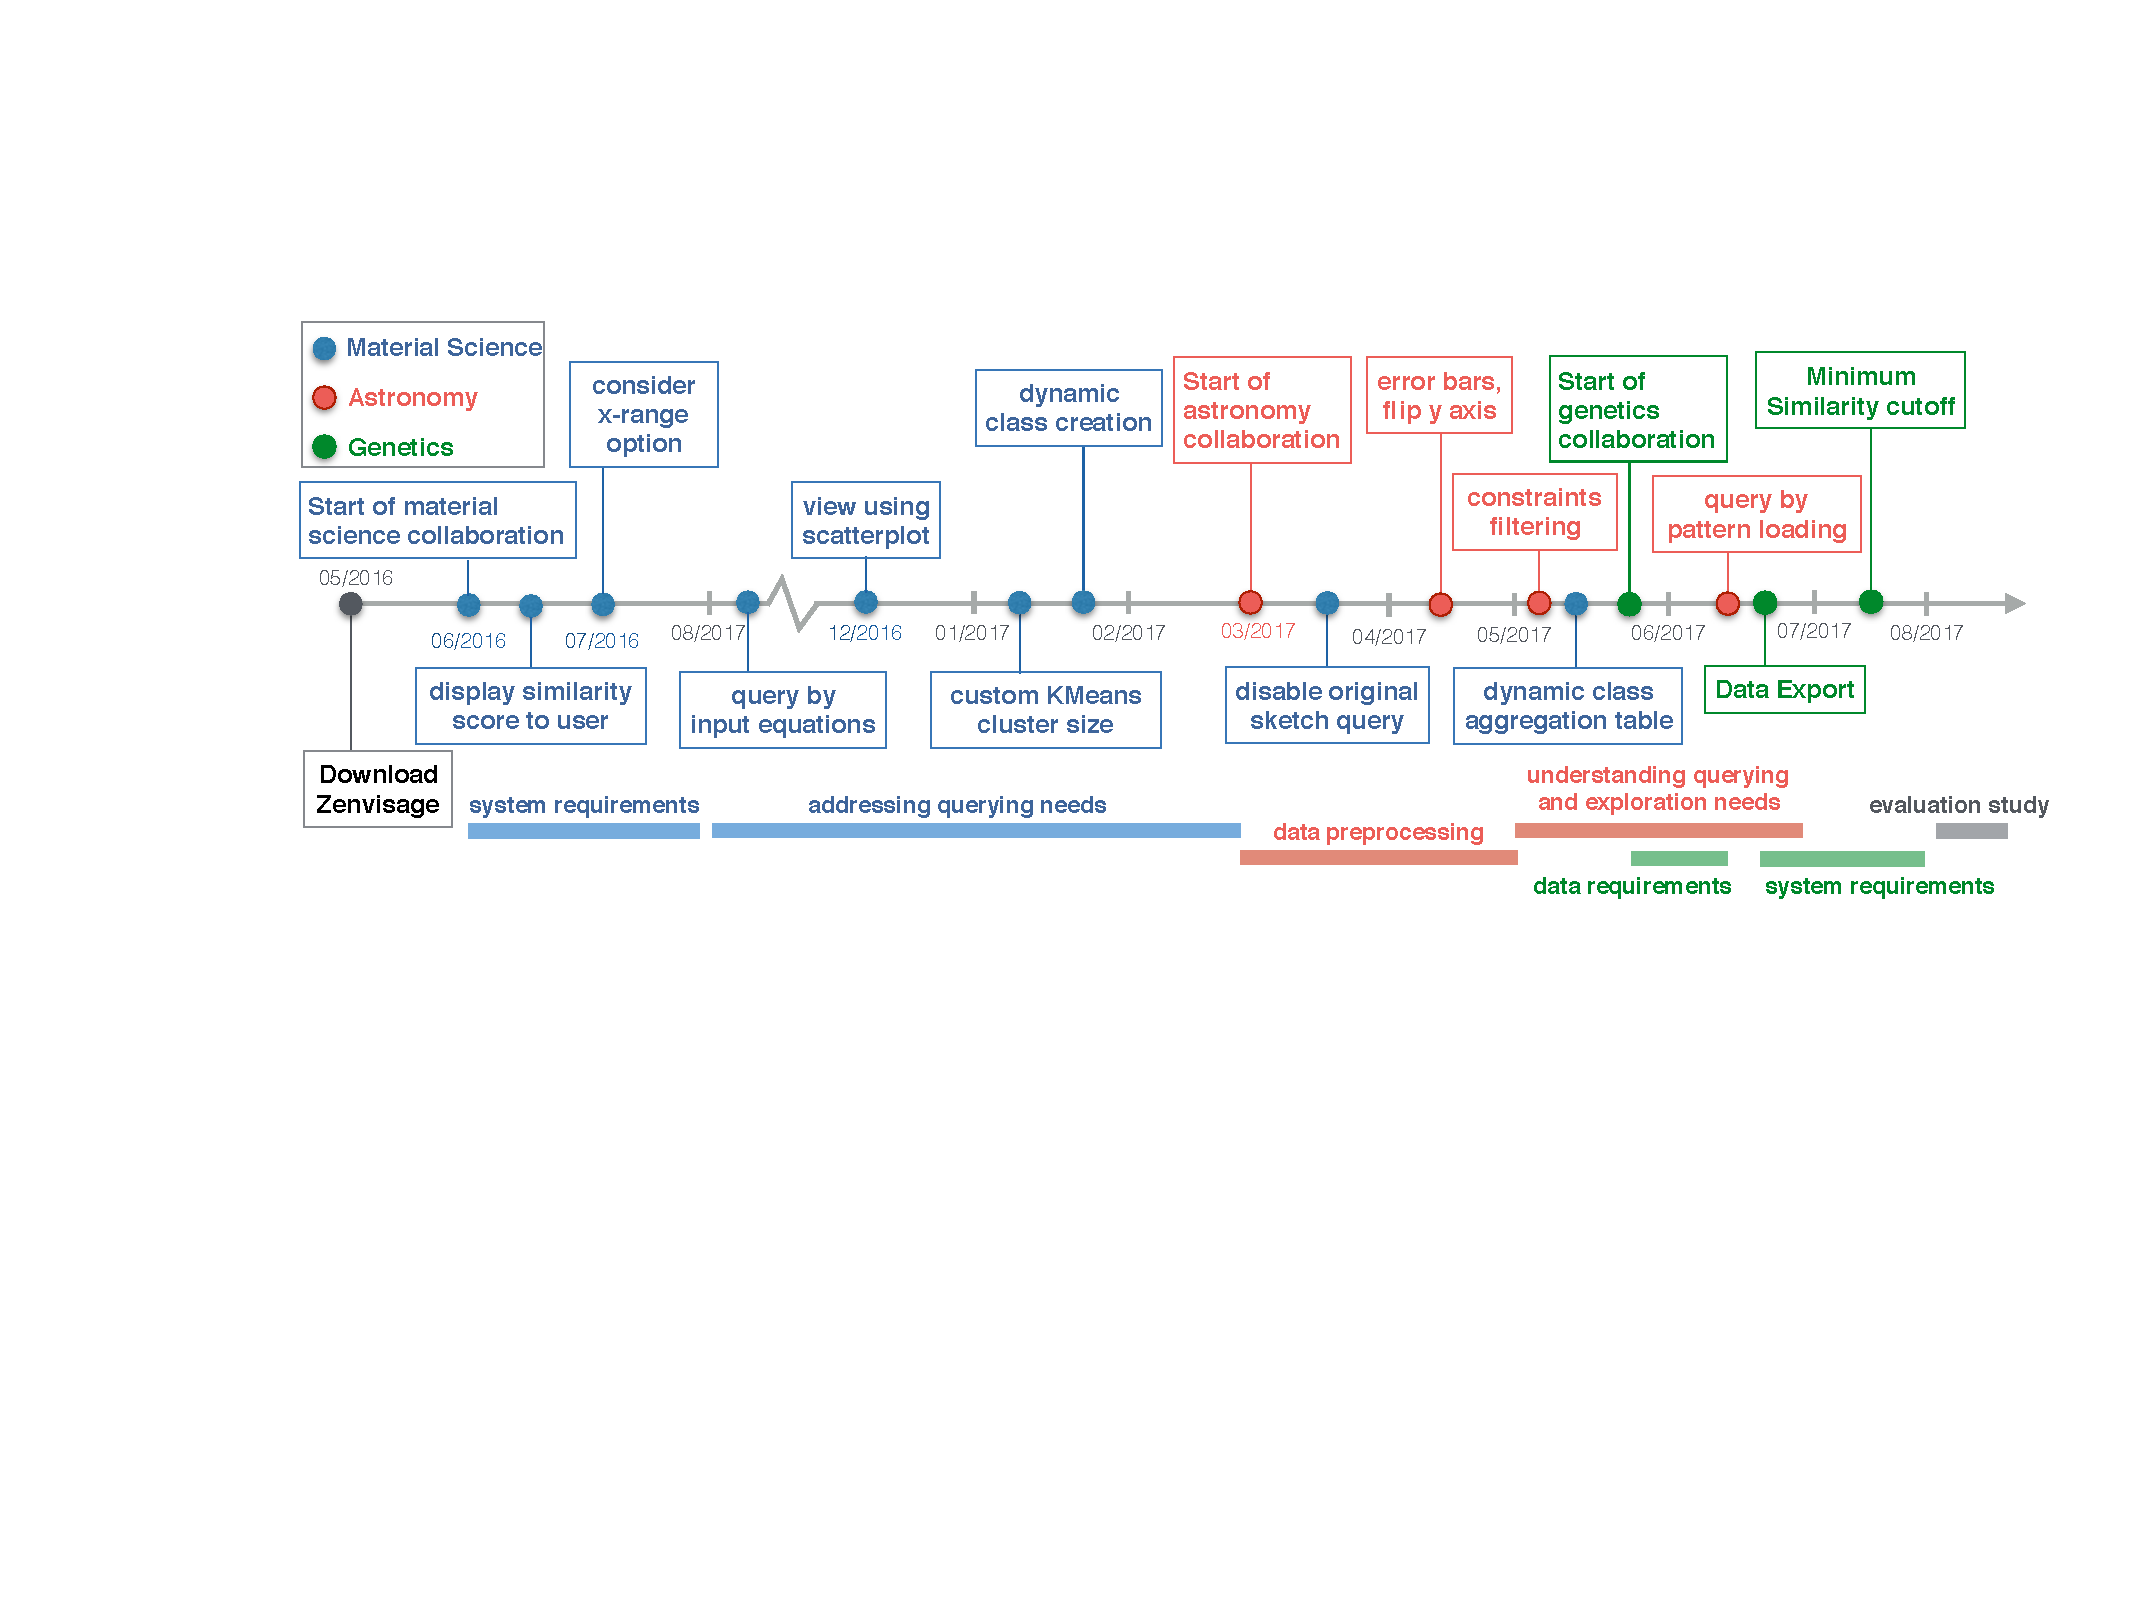
\includegraphics[width=6in]{figures/timeline_anon.pdf}
	\vspace{-6pt}\caption{Timeline for progress in participatory design studies.}
	\label{timeline}
	\vspace{-10pt}
\end{figure*}
\par Via cognitive walkthroughs and interviews, we first identified challenges in existing data analysis workflows in these domains
that could be potentially addressed by a VQS. Building on top of an existing, open-source VQS, \zv~\cite{Siddiqui2017,Siddiqui2017VLDB}, we collaborated closely with our participants to gather feedback and iterate on VQS feature designs,
over the course of a year, culminating in a new enhanced VQS, \zvpp. We organized these features into a taxonomy of VQS functionalities, involving three sensemaking processes inspired by Pirolli and Card's notional model of analyst sensemaking~\cite{Pirolli}. The sensemaking processes include top-down pattern specification (translating a pattern ``in-the-head'' into the form of a visual query), bottom-up data-driven inquiries (querying or recommending based on data), and context-creation (navigating across different collections of visualizations). We find that prior VQSs have focused largely on top-down processes, while largely ignoring the other two processes that are crucial for the needs in all three domains.
\par To study how various VQS features
are used in practice,
we conducted a final evaluation study with nine participants
using our final VQS prototype, \zvpp,
to address their research questions
on their own datasets.
In a 1.5-hour user study, participants were able to
gain novel scientific insights,
such as identifying a star with a transient pattern
that was known to harbor a Jupiter-sized planet
and finding characteristic gene expression profiles confirming the results of a related publication.\techreport{, and discovering that the dip in an astronomical light curve is caused by saturated imaging equipment overlooked by the existing error-detection pipeline.} \techreport{Participants also gain additional insights about their datasets, including debugging mislabeled features and uncovering erroneous data preprocessing procedure applied to a collaborator's dataset.}
%that goes from a pattern in-the-head to a desired visualization

\par By analyzing the evaluation study results, we discovered that sketching a pattern for querying is often ineffective. This is due to the fact that sketching makes the problematic assumptions that users know the pattern that they want to sketch and are able to sketch it precisely. Instead, participants typically opted for other means of pattern specification---one common mechanism was to drag-and-drop a recommended pattern onto the canvas, and then modify it (e.g., by smoothing it out). However, most VQSs do not support these other mechanisms (as we argued earlier, they typically focus only on top-down sensemaking processes, without covering bottom-up and context creation), partially explaining why such systems have not been widely adopted in practice.
\par Further analysis of how participants
transition between different sensemaking processes
during analysis---including the construction of a Markov Model---illustrated
how participants adopt a diverse set of workflows tailored
to their domains. We find that participants often construct analysis workflows focused around a primary sensemaking process, while iteratively interleaving their analysis with the two other processes. This finding points to how all three sensemaking processes, along with seamless transitions between them, are essential for enabling users to effectively use VQSs for data exploration.%For example, participants often center on a main sensemaking process, while interleaving variations with other two processes as they iterate on an analytic task.
\par To the best of our knowledge, our study is the \emph{first to holistically examine how VQSs can be designed to fit the needs of real-world
analysts and how they are actually used in practice}. Our contributions include:
\begin{denselist}
\item a characterization of the problems addressable by VQSs through design studies with three different domains,
\item the construction of a taxonomy of functionalities within VQSs, as well as an articulation of the problem space that is amenable to VQSs, both grounded in participatory design findings,
\item \change{an integrative} VQS, \zvpp, capable of facilitating rapid hypothesis generation and insight discovery,
\item study findings on how VQSs are used in practice, leading to the development of a novel sensemaking model for VQSs. %including the ineffectiveness of
%evaluation
% sketching and the ---- workflow
\end{denselist}
Our work not only opens up a new space of opportunities beyond the narrow use cases considered by prior studies, but also advocates common design guidelines and end-user considerations for building next-generation VQSs.
 %From these experiences, we  advocate visualization researchers and tool designers to ---- future VQS opportunities  Understanding the design space and opportunities for VQS
% Our three main research questions are as follows:

%and not as commonly ---- due to the --- challenges ----. that ----- characteristic workflows ---- iterative sensemaking loop.
%Our collaborative design experience culminated in a full-fledged VQS, \zvpp, described in Section~\ref{sec:pd_findings}.
% \noindent \emph{RQ1: What are the challenges in existing scientific data analysis workflows that could be potentially addressed by a VQS?}
% \par Via cognitive walkthroughs and interviews,
% we gained an understanding of the data analysis
% workflows presently employed by the scientists, their needs,
% and the challenges they face.
% We identified opportunities where a VQS could
% help accelerate their analysis, by helping them
% discover insights, gain intuition, or provoke directions
% for exploration. Finally, we determined the types of
% research questions and dataset properties that would
% be most suitable for exploration on VQSs.
%By learning about the needs and challenges that scientists face when working with their datasets through interviews and cognitive walkthroughs, we learned about the types of queries that they would like to pose on VQSs and distilled a set of design specifications that can better enable VQSs to help them discover insights, gain intuition about their datasets or provoke further directions for exploration. We also identify the types of research questions and dataset properties would be suitable for data exploration on VQSs.
% \begin{figure*}[ht!]
% \centering
% \vspace{-15pt}
% 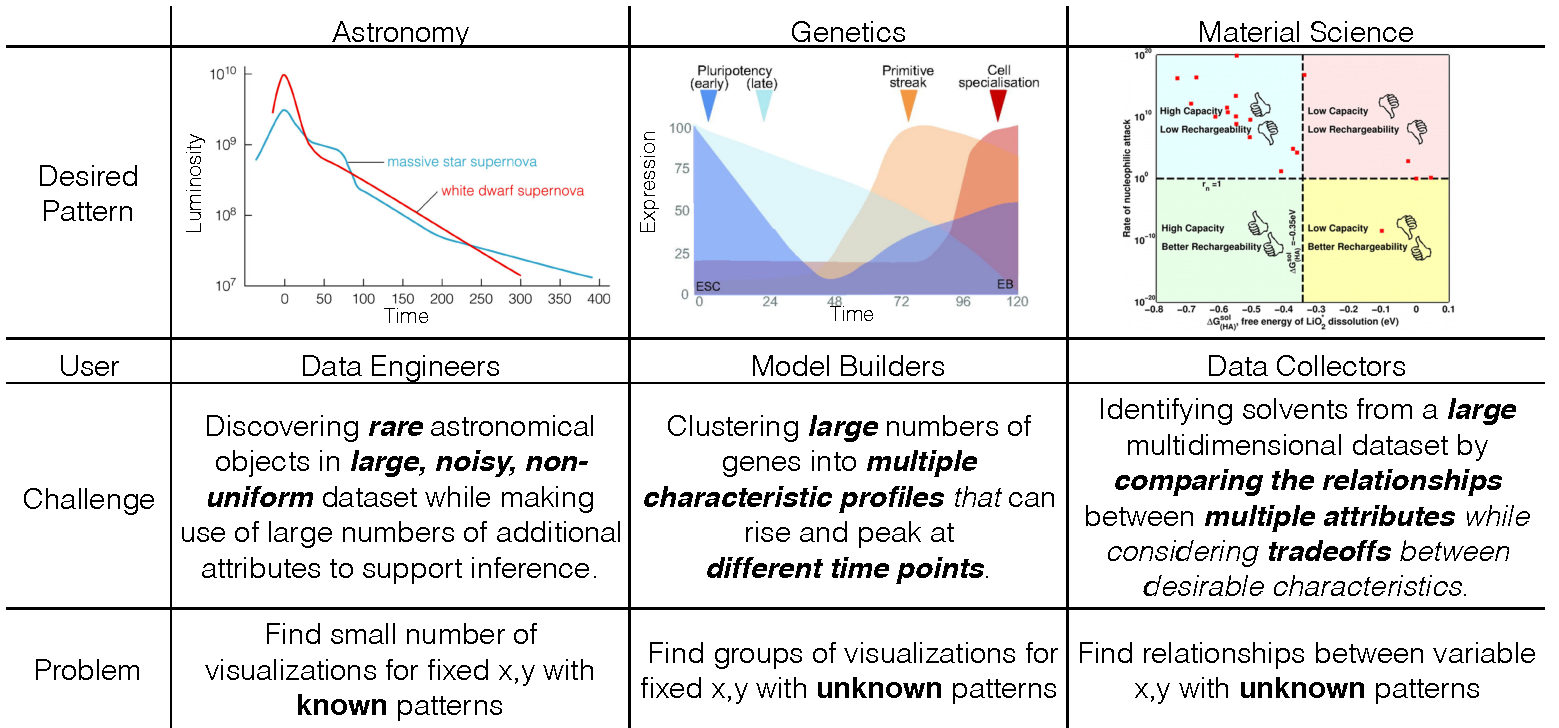
\includegraphics[width=0.8\linewidth]{figures/sci_challenge_tbl.pdf}
% \vspace{-6pt}\caption{Descriptions of the three scientific use cases discussed in this paper.}
% \label{example}
% \vspace{-10pt}
% \end{figure*}

% \noindent \emph{RQ2: What types of interface capabilities are necessary to develop VQSs into a useful component of data analysis?}
% \par Via participatory design, we distilled
% \tvcg{Based on our early interactions with scientists,
% we started to build a VQS~\cite{Siddiqui2017VLDB,Siddiqui2017} that, similar to existing VQSs~\cite{wattenberg2001sketching}, allowed them to search for desired trends via drawing on a canvas. This early system served as a functional prototype for us to engage with scientists further in the participatory design process, understand how they envision themselves using a VQS, and gather feedback on feature designs that could make the VQS more useful. The features we developed address challenges shared across the three scientific domains, ranging from additional querying modalities, to features that support a more integrated workflow, to improving the interpretability of the system output, \tvcg{most of them missing in} prior VQSs in the literature. Our collaborative design experience culminated in a full-fledged VQS, \zv, capable of facilitating rapid hypothesis generation and insight discovery.}

% \noindent \emph{RQ3: How do VQSs accelerate scientific insights?} and \emph{RQ4: How can VQSs fit within the context of existing data analysis workflows?}
% \\ To evaluate our final system \zv, we conducted a user study with nine scientists (including those who had participated in the design process), all of whom had a vested interest in using a VQS to address their research questions on their datasets. In a 1.5-hour user study, our scientist participants were able to gain novel scientific insights, such as \emph{\tvcg{identifying a star with a transient pattern that was known to harbor a Jupiter-sized planet,} finding characteristic gene expression profiles that confirmed the results of a related publication, and learning that the dip in an astronomical light curve is caused by saturated imaging equipment overlooked by the existing error-detection pipeline}.  Participants also gained additional insights about their datasets, including debugging \tvcg{mislabelled features and uncovering the erroneous data preprocessing procedure applied to a collaborator's dataset.}
% that the way data is aggregated across multiple experiments is erroneous on a collaborator's dataset.
% We learned how VQSs could be contextualized within scientific data analysis workflows and discovered that VQSs can be used beyond the exploratory phase of analysis, for data verification, debugging preliminary datasets, and performing sanity-checks on downstream models.

% \begin{figure}[h!]
%     \centering
%     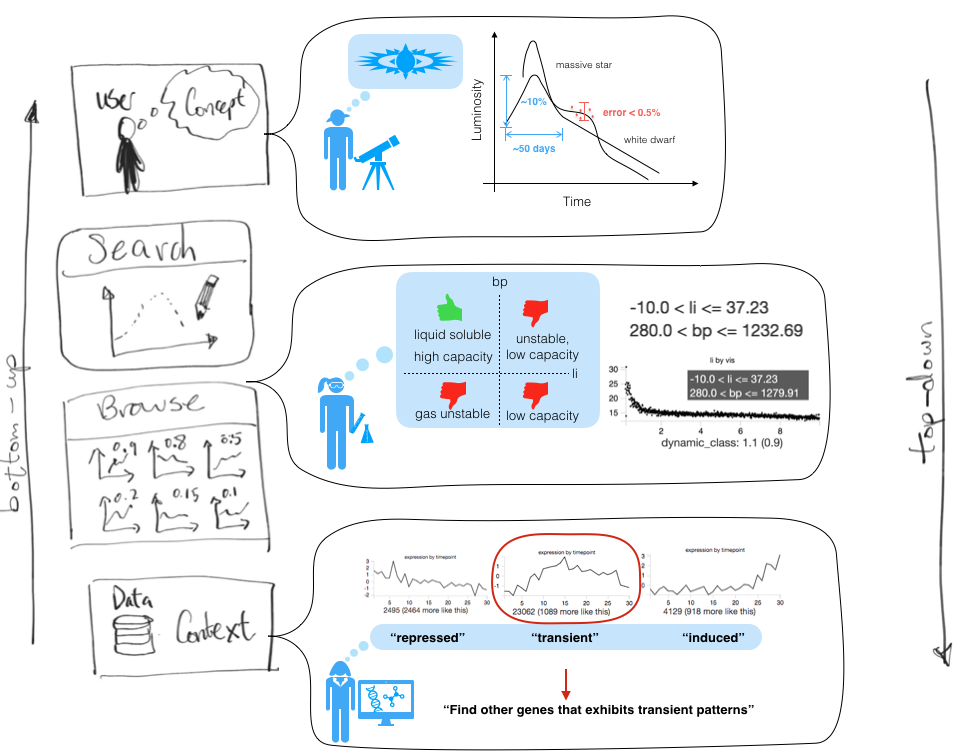
\includegraphics[width=\linewidth]{figures/search-browse-model.png}
%     \vspace{-6pt}\caption{Search Browse Model}
%     \label{fig:sbmodel}
%     \vspace{-5pt}
% \end{figure}

%!TEX root = main.tex
\section{Methods\label{sec:methods}}
\subsection{Background and Motivation}
\par Visual query systems enable users to directly search for visualizations matching certain patterns through an intuitive specification interface. Early work in this space focused on interfaces to search for time series of interest, including TimeSearcher~\cite{Hochheiser2001,Hochheiser2004}, where the query is composed of one or more rectangular value-range selections, and QuerySketch~\cite{wattenberg2001sketching} and Google Correlate~\cite{mohebbi2011google}, where the query is sketched as a pattern. Subsequent work recognized the ambiguity of sketches and improved the expressiveness of sketched queries through finer specification interfaces and pattern-matching algorithms~\cite{ryall2005querylines,Holz2009}, as well as performed crowdsourced perceptual studies to understand how humans rank similarity in patterns subjectively~\cite{Eichmann2015,correll2016semantics,Mannino2018}. Table~\ref{table:relatedwork} summarizes the list of features offered by these existing systems.
% , including the use of soft constraints~\cite{ryall2005querylines} and implicit relaxed selection techniques~\cite{Holz2009}. 
% In addition to this ongoing work, recent work have also performed crowdsourced perceptual studies to understand how humans rank similarity in patterns subjectively~\cite{Eichmann2015,correll2016semantics,Mannino2018}. 
\begin{table*}[ht!]
    \begin{tabular}{l
    >{\columncolor[HTML]{67FD9A}}l
    >{\columncolor[HTML]{67FD9A}}l
    >{\columncolor[HTML]{67FD9A}}l
    >{\columncolor[HTML]{67FD9A}}l
    >{\columncolor[HTML]{FD6864}}l
    >{\columncolor[HTML]{FD6864}}l
    >{\columncolor[HTML]{FD6864}}l
    >{\columncolor[HTML]{FD6864}}l
    >{\columncolor[HTML]{FD6864}}l }
                                                      & \multicolumn{1}{c}{\cellcolor[HTML]{DAE8FC}{\color[HTML]{000000}  \thead{Freehand \\ Sketching}}} & \multicolumn{1}{c}{\cellcolor[HTML]{DAE8FC}{\color[HTML]{000000}  \thead{Shape \\ Approx.}}} & \multicolumn{1}{c}{\cellcolor[HTML]{DAE8FC}{\color[HTML]{000000}  \thead{Range \\ Selection}}} & \multicolumn{1}{c}{\cellcolor[HTML]{DAE8FC}{\color[HTML]{000000} \thead{Flexible\\ Matching}}} & \multicolumn{1}{c}{\cellcolor[HTML]{FFCE93}{\color[HTML]{000000} \thead{Filter \\ Selection}}} & \multicolumn{1}{c}{\cellcolor[HTML]{FFCE93}{\color[HTML]{000000} \thead{Group\\ Comparison}}} & \multicolumn{1}{c}{\cellcolor[HTML]{FFFFC7}\thead{Concept\\ Querying}} & \multicolumn{1}{c}{\cellcolor[HTML]{FFFFC7}\thead{Result\\ Querying}} & \multicolumn{1}{c}{\cellcolor[HTML]{FFFFC7}\thead{Recommend \\ Result}} \\
    Timesearcher \cite{Hochheiser2001,Hochheiser2004} & \cellcolor[HTML]{FD6864}{\color[HTML]{000000} }                                        &                                                                                                                               &                                                                                                                                & \cellcolor[HTML]{FD6864}{\color[HTML]{FE0000} }                                       & {\color[HTML]{FE0000} }                                                              & {\color[HTML]{FE0000} }                                                              & {\color[HTML]{FE0000} }                                       & \cellcolor[HTML]{67FD9A}                                     & {\color[HTML]{FE0000} }                                    \\
    QuerySketch \cite{wattenberg2001sketching}        &                                                                                        & \cellcolor[HTML]{FD6864}                                                                                                      &                                                                                                                                & \cellcolor[HTML]{FD6864}                                                              &                                                                                      &                                                                                      &                                                               &                                                              &                                                            \\
    QueryLines \cite{ryall2005querylines}             &                                                                                        &                                                                                                                               &                                                                                                                                &                                                                                       &                                                                                      &                                                                                      &                                                               &                                                              &                                                            \\
    SoftSelect \cite{Holz2009}                        &                                                                                        &                                                                                                                               & \cellcolor[HTML]{FD6864}                                                                                                       &                                                                                       &                                                                                      &                                                                                      &                                                               &                                                              &                                                            \\
    Google Correlate \cite{mohebbi2011google}         & \cellcolor[HTML]{67FD9A}                                                               & \cellcolor[HTML]{FD6864}                                                                                                      & \cellcolor[HTML]{FD6864}                                                                                                       &                                                                                       &                                                                                      &                                                                                      & \cellcolor[HTML]{67FD9A}                                      &                                                              & \cellcolor[HTML]{67FD9A}                                   \\
    TimeSketch \cite{Eichmann2015}                    &                                                                                        & \cellcolor[HTML]{FD6864}                                                                                                      & \cellcolor[HTML]{FD6864}                                                                                                       & \cellcolor[HTML]{FD6864}                                                              &                                                                                      &                                                                                      &                                                               &                                                              &                                                            \\
    SketchQuery \cite{correll2016semantics}           &                                                                                        &                                                                                                                               & \cellcolor[HTML]{FD6864}                                                                                                       &                                                                                       &                                                                                      &                                                                                      &                                                               & \cellcolor[HTML]{67FD9A}                                     &                                                            \\
    Qetch \cite{Mannino2018}                          &                                                                                        &                                                                                                                               &                                                                                                                                &                                                                                       &                                                                                      &                                                                                      &                                                               &                                                              & \cellcolor[HTML]{67FD9A}                                   \\
    Zenvisage                                         &                                                                                        &                                                                                                                               &                                                                                                                                &                                                                                       & \cellcolor[HTML]{67FD9A}                                                             & \cellcolor[HTML]{67FD9A}                                                             & \cellcolor[HTML]{67FD9A}                                      & \cellcolor[HTML]{67FD9A}                                     & \cellcolor[HTML]{67FD9A}
    \end{tabular}
    \caption{Table summarizing the key components of VQSs (columns) covered by past systems (row). Green indicates that feature exist in the system; red indicate feature not covered. Column header colors blue, orange, yellow covers processes: top-down querying, search with context, and bottom-up querying respectively, described more in Section~\ref{sec:guidelines}. }
\end{table*}

\par While these systems have been shown to be effective for visual querying in controlled lab studies, they have not been evaluated in-situ on real-world use cases. In this work, we adopted a mixed methods research methodology that draws inspiration from ethnographic methods, iterative and participatory design, and controlled studies~\cite{Plaisant2004,lam2012empirical,miller_salkind_miller_2002,shneiderman2006strategies,Muller1993} to more thoroughly understand the design space of VQSs and how various components of VQSs are used in practice. Participatory design has been successfully used in the development of interactive visualization systems in the past~\cite{Aragon2008,Chuang2012}. Sedlmair et al. \cite{Sedlmair2012} advocate that design study methodology is suitable for use cases in which the data is available for prototyping, but the task is only partially known and the information is partially in the user's head. %to understand how VQSs can be used in scientific data analysis. %In that regard, our scientific use cases with VQS is well-suited for a design study methodology, as we learn about the scientist's data and analysis requirements and design interactions that helps users translate their ``in-the-head'' specifications into actionable visual queries.
\subsection{Participatory Design}
\par  Working with researchers from three different scientific research groups, we identified the needs and challenges of scientific data analysis and potential opportunities for VQSs, via interviews and cognitive walkthroughs. We recruited participants by reaching out to research groups via email and word of mouth, who have experienced challenges in dealing with large amounts of data. We initially spoke to analysts from 12 different potential application areas and narrowed down to three use cases in astronomy, genetics, and material science for our participatory design study, based on their suitability for VQS as well as diversity in use cases. Six scientists from three research groups participated in the design of \zv. On average, participants had more than 8 years of research experience working in their respective fields. %\techreport{We list the participants in Table~\ref{participants}, and will refer to them by their anonymized ID as listed in the table throughout the paper.}
\par Given our early conversations with participants, we built a basic VQS to serve as the functional prototype in the design study. This early VQS prototype allowed users to sketch a pattern or drag-and-drop an existing visualization as a query, then the system would return visualizations that had the closest Euclidean distance from the queried pattern. The details of the system is described in \cite{Siddiqui2017,Siddiqui2017VLDB}, which focused on the system and scalability aspects of the VQSs.
	% \begin{figure}[ht!]
	% \centering
	% 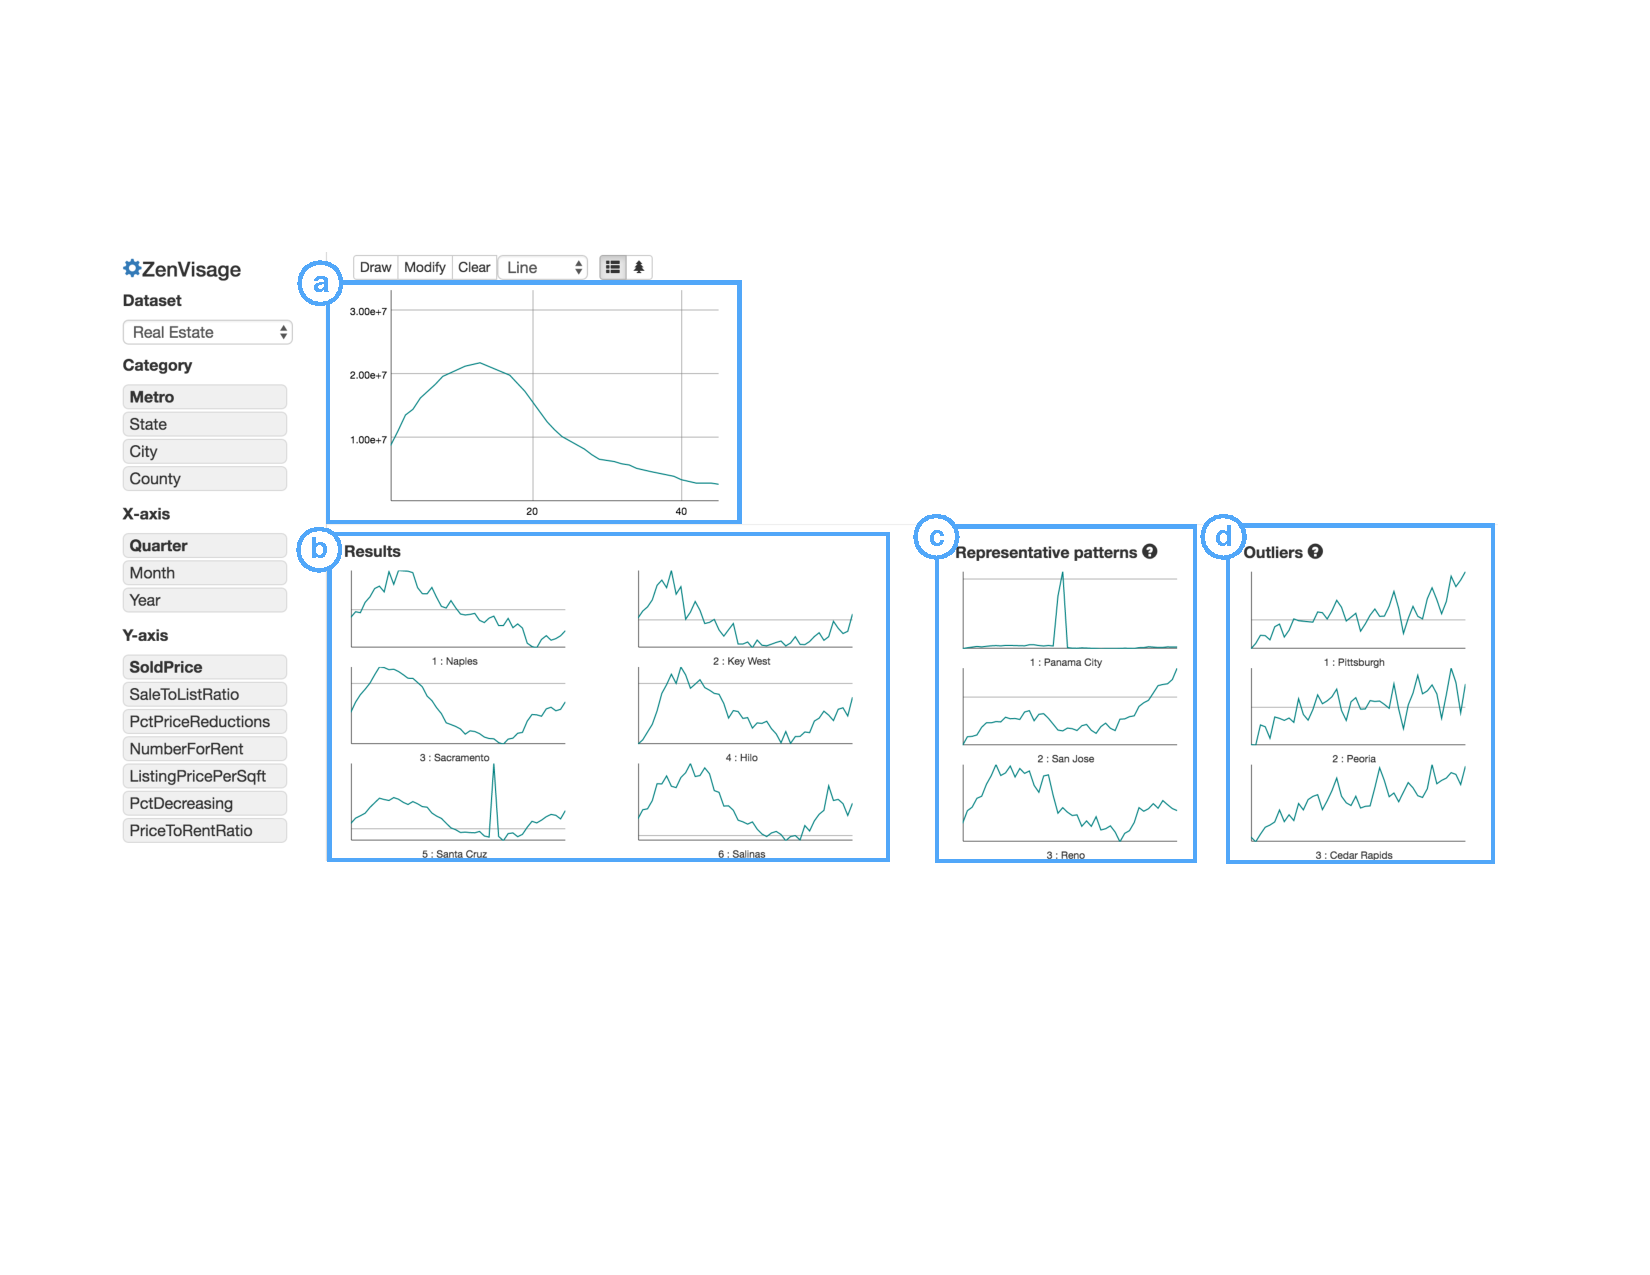
\includegraphics[width=\linewidth]{figures/oldZV_nozql.pdf}
	% \caption{The \zv prototype allowed users to sketch a pattern in (a), which would then return (b) results that had the closest Euclidean distance from the sketched pattern. The system also displays (c) representative patterns obtained through K-Means clustering and (d) outlier patterns to help the users gain an overview of the dataset.}
	% \label{oldZV}
	% \end{figure}
\par The use of functional prototypes is common and effective in participatory design to provide a starting point for the participants, as studied by Ciolfi et al.\cite{Ciolfi2016}. %For example, Ciolfi et al.\cite{Ciolfi2016} studied two different alternatives to co-design (starting with open brief versus functional prototype) in the development of museum guidance systems and found that while both approaches were equally fruitful, functional prototypes can make addressing a specific challenge more immediate and focused. 
Our motivation for providing a functional prototype at the beginning of the participatory design sessions is to showcase capabilities of VQSs. Especially since VQSs are not common in the existing workflows of these scientists, participants may not be able to imagine their use cases without a starting point.
\par During the participatory design process, we collaborated with each of the teams closely with an average of two meetings per month, where we learned about their datasets, objectives, and how VQSs could help address their research questions. A summary timeline of our engagement with the participants and the features inspired by their use cases can be found in Figure \ref{timeline}. Participants provided datasets they were exploring from their domain, whereby they had a vested interest in using a VQS to address their own research questions. Through this process, we identified and incorporated more than 20 desired features into our VQS prototype, \zv, over the period of a year.
\begin{figure*}[!ht]
	\centering
	\captionsetup{justification=centering,margin=2cm}
	\vspace{-10pt}
	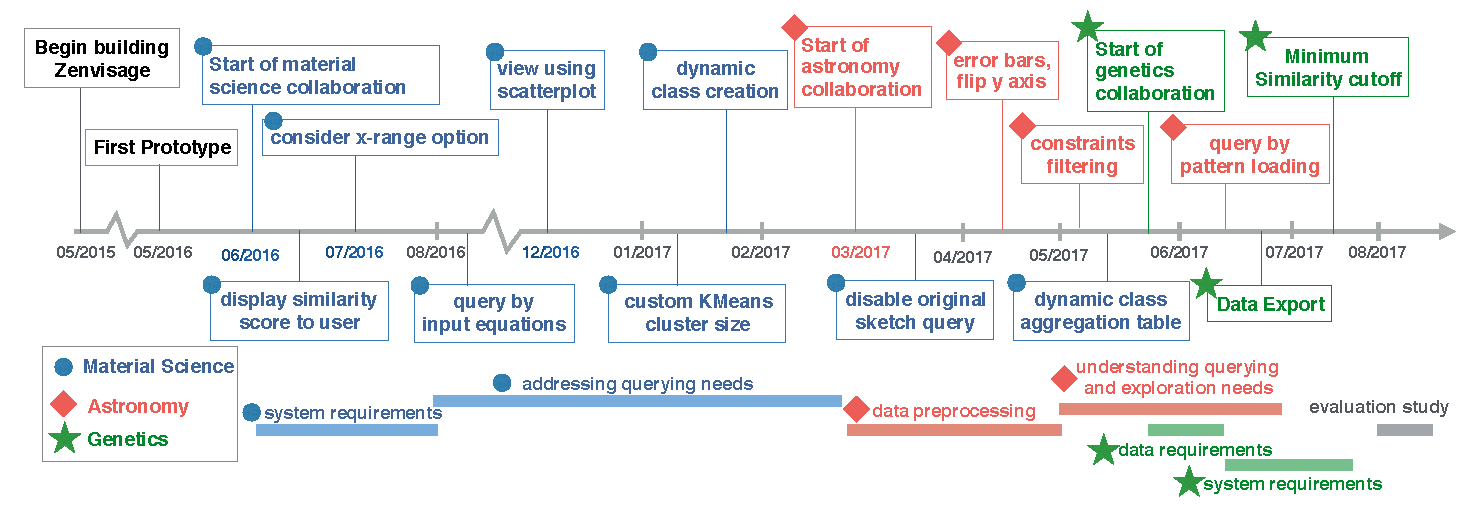
\includegraphics[width=6in]{figures/timeline_new.pdf}
	\vspace{-6pt}\caption{Participatory design timeline for the scientific use cases.}
	\label{timeline}
	\vspace{-10pt}
\end{figure*}
\subsection{Evaluation Study}
\par Visualization systems are often evaluated using controlled studies that measure the user's performance against an existing visualization baseline~\cite{Plaisant2004}. Techniques such as artificially inserting ``insights'' or setting predefined tasks for example datasets work well for objective tasks, such as debugging data errors~\cite{kandel2011wrangler,Patel2010}, but these contrived methods are unsuitable for trying to learn about the types of real-world queries users may want to pose on VQSs. %Due to the unrealistic nature of controlled studies, many have proposed using a more multi-faceted, ethnographic approach to understand how analysts perform visual data analysis and reasoning~\cite{Plaisant2004,lam2012empirical,shneiderman2006strategies,munzner2009nested,Sedlmair2012}. 
In order to make the evaluation more realistic, at the end of our participatory design study, we opted for a qualitative evaluation where we invited participants to bring datasets that they have vested interests in to address unanswered research questions, in order to study how analysts interact with different VQS components in practice.
\par The evaluation study participants included the six scientists from participatory design, along with three additional ``blank-slate'' participants who had never encountered \zv before. While participatory design subjects actively provided feedback on \zv with their data, they only saw us demonstrating their requested features and explaining the system to them, rather than actively using the system on their own. So the evaluation study was the first time that all participants used \zv to explore their datasets.
\par Participants for the evaluation study were recruited from each of the three aforementioned research groups, as well as domain-specific mailing lists. Prior to the study, we asked the potential participants to fill out a pre-study survey to determine their eligibility. Eligibility criteria included: being an active researcher in the subject area with more than one year of research experience, and having worked on a research project involving data of the same nature as that used in the participatory design. Four of the evaluation studies were conducted remotely. Participants had the option of exploring their own dataset or an existing dataset that they provided to us during the participatory design process. All three blank-slate participants opted to explore their own datasets. %After loading their dataset, we emailed them a screenshot of a visualization from our tool to verify that we configured the system to meet their needs.
\par At the start, participants were provided with an interactive walk-through explaining the system details and given approximately ten minutes to experience a guided exploration of our VQS with a preloaded real-estate example dataset from Zillow \cite{zillow}.\techreport{This dataset contained housing data for various cities, metropolitan areas, and states in the U.S. from 2004-15.} After familiarizing themselves with the tool, we loaded the participant's dataset and encouraged them to talk-aloud or use external tools as needed during the data exploration phase.% and suggested an appropriate choice of axis to begin the exploration. 
%\par During the exploration phase, participants were informed that they could use other tools as needed. 
If the participant was out of ideas\ccut{ for three minutes}, we suggested one of the ten main functionalities in \zv \techreport{\footnote{query by sketching, drag-and-drop, pattern loading, input equations, representative and outliers, narrow/ignore x-range options, filtering, data smoothing, creating dynamic classes,  data export}}that they had not yet used. If any of these operations were not applicable to their specific dataset, they were allowed to skip the operation after having considered how it may or may not be applicable to their workflow. The user study ended after they covered all ten main functionalities. On average, the main exploration phase lasted for 63 minutes. After the study, we asked them open-ended questions about their experience.
%!TEX root = main.tex
\section{Participants and Datasets\label{sec:participantdatasets}}
At the start of our design study, \change{we conducted contextual inquiry to learn about our participants'} existing data analysis workflows. Next, we describe our study participants\change{, their scientific goals, } and their preferred analysis workflows. \change{Note that while we have collaborated with each application domain in depth, due to the space limitation of the paper, we summarize the key findings in each domain to highlight their commonalities and differences, in order to provide a backdrop for generalized VQSs findings described later in the paper.}
%use cases to highlight behaviors that participants have adopted for conducting certain analysis tasks.
\par\noindent\stitle{Astronomy:} The Dark Energy Survey is a multi-institution project that surveys 300 million galaxies over 525 nights to study dark energy~\cite{Drlica-Wagner2017}. The telescope used to survey these galaxies also focuses on smaller patches of the sky on a weekly interval to discover astronomical transients (objects whose brightness changes dramatically as a function of time), such as supernovae or quasars. Their dataset consists of a large collection of \change{\emph{light curves}: brightness observations over time, one associated with each astronomical object, plotted as time series. Over} five months, we worked closely with A1, an astronomer on the project's data management team working at a supercomputing facility. Their scientific goal is to identify potential astronomical transients in order to study their properties. \techreport{These insights can help further constrain physical models regarding the formation of these objects.}
\npar To identify transients, astronomers programmatically generate visualizations of candidate objects with \texttt{matplotlib} and visually examine each light curve. While an experienced astronomer who has examined many transient light curves can often distinguish an interesting transient object from noise by sight, manual searching for transients is time-consuming and error prone, since the large majority of the objects are false positives. A1 was interested in VQSs as he recognized how specific pattern queries could help astronomers directly search for these rare transients.
\techreport{\par If an object of interest or region is identified through the visual analysis, then the astronomer may be interested in inspecting the image of the region for cross-checking that the significant change in brightness of the object is not due to an imaging artifact. This could be done using a custom built web-interface that facilitates the access of cutout images for a queried region of the sky.}
\par\noindent\stitle{Genetics:} Gene expression is a common measurement in genetics obtained via microarray experiments~\cite{Peng2016}. \techreport{In these experiments, a grid containing thousands of DNA fragments are exposed to stimuli and measurements for the level at which a gene is expressed are recorded as a function of time.} We worked with a graduate student (G1) and professor (G3) at a research university who were using gene expression data to understand how genes are related to phenotypes expressed during early development\techreport{\cite{Peng2016,Gloss2017}}. Their data consisted of a collection of gene expression profiles over time for mouse stem cells, aggregated over multiple experiments.\techreport{, downloaded from an online database\footnote{\url{ncbi.nlm.nih.gov/geo/}}.} %They were interested in using \zv to cluster gene expression data before conducting analysis with a downstream machine learning workflow.
\npar Their typical workflow is as follows: G1 first loads the preprocessed gene expression data into a custom desktop application for visualizing and clustering it\techreport{\footnote{\url{www.cs.cmu.edu/~jernst/stem/}}}. After setting several system parameters and executing the clustering algorithm, the overlaid time series for each cluster is displayed on the interface. G1 visually inspects that the patterns in each cluster looks ``clean'' and checks that the number of outlier genes (i.e., those that do not fall into any of the clusters) is low.  If the number of outliers is high or the clustered visualizations look ``unclean'', she reruns the analysis by increasing the number of clusters. Once the visualized clusters look ``good enough'', G1 exports the clusters to her downstream regression tasks.
\npar Prior to the study, G1 and G3 spent over a month attempting to determine the best number of clusters based on a series of static visualizations and statistics computed after clustering. While regenerating their results took no more than 15 minutes every time they made a change, the multi-step, segmented workflow meant that all changes had to be done offline.\techreport{, so that valuable meeting time was not wasted trying to regenerate results.} \change{They were interested in VQSs as interactively querying time series with clustering results could dramatically speed up their collaborative analysis process.}
%The team were interested in VQSs as they saw how interactively querying time series with clustering results could dramatically speed up their collaborative analysis process.
%that can improve battery performance and stability
\par\noindent\stitle{Material Science:} We collaborated with material scientists at a research university who are working to identify solvents for energy efficient and safe batteries. These scientists work on a large simulation dataset containing chemical properties for more than 280,000 solvents~\cite{Khetan2018}. Each row of their dataset represents a unique solvent with 25 different chemical attributes. We worked closely with a a postdoctoral researcher (M1), professor (M2), and graduate student (M3) for over a year to design a sensible way of exploring their data. They wanted to use VQSs to identify solvents that not only have similar properties to known solvents\change{,} but are also more favorable (e.g., cheaper or safer to manufacture). To search for these desired solvents, they need to understand how changes in certain chemical attributes affect other properties under specific conditions.
\npar M1 typically starts his data exploration process by iteratively applying filters to a list of potential battery solvents using SQL queries. \change{Once the remaining solvent list is sufficiently small, each solvent is examined in more detail to factor in its cost and availability to determine experimental feasibility. They} were interested in VQSs as it was impossible for them to uncover hidden relationships between different attributes across large number of solvents manually.%(such as how changing one attribute affects another attribute)

%!TEX root = main.tex
\begin{figure*}[ht!]
\centering
\vspace{-15pt}
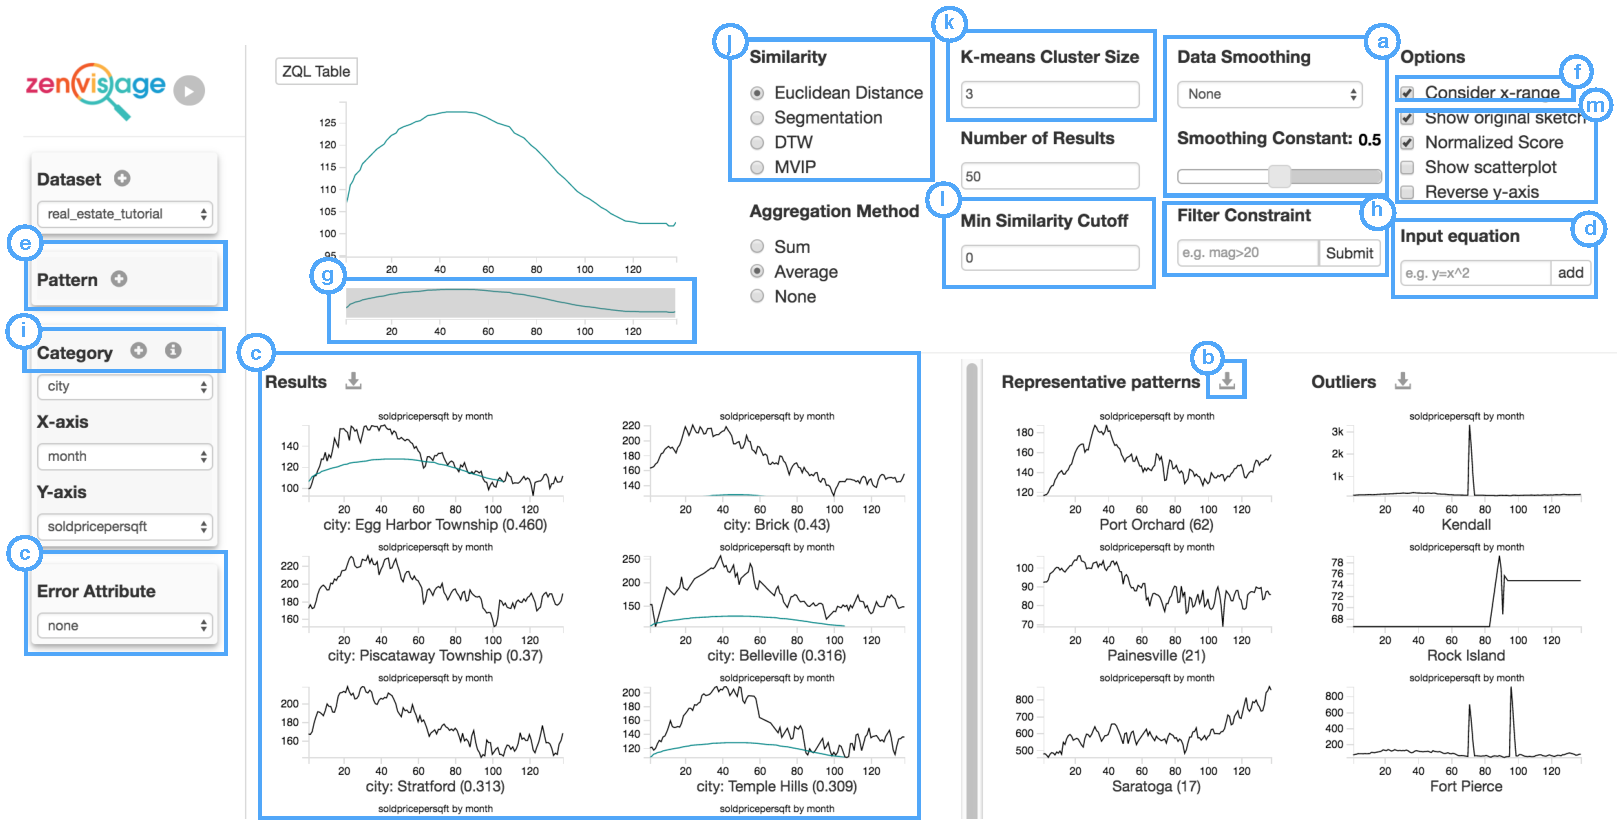
\includegraphics[width=\linewidth]{figures/newZV.pdf} %5.5
\vspace{-5pt}\caption{Our VQS after participatory design, which includes: querying functionalities via (a) patterns and (n) equations; query specification mechanisms including  (b) Dynamic class creation, (j) Filtering, and  (e) x-range invariance, selection and filtering; the ability to preprocess via (i) interactive smoothing; visualization display options (c); system parameter options (g, i, f); and the ability to export data outputs. Prior to the participatory design, \zv only included a single sketch input with no additional options. \zv also displayed representative patterns and outlier patterns.}
\label{zvOverview}
\vspace{-14pt}
\end{figure*}

\section{Themes Emerging from Participatory Design (R2)}\label{findings}
\par In the previous section, we gained an understanding of the current analysis workflows employed in the three use cases. Next, to address RQ2, we employed participatory design with our scientists to incorporate key features  missing in our original VQS, and unaddressed in their
current workflows.  Of the 20 features we implemented, 16 were suggested by multiple use cases. We discovered three central themes
encapsulating these features that are important to facilitate rapid
hypothesis generation and insight discovery, but are missing in prior VQSs,  described next. 
While some of our findings echo prior work on system-level taxonomies of visualization tasks \cite{Amar2005,Heer2012}, we highlight how specific analytic tasks and interaction features could be used to enhance VQSs in particular. \techreport{In particular, we learned that \textit{participants wanted more control over the internals of the systems and an integrated workflow that helped streamline their analysis when using VQSs.}}
\subsection{Uninterrupted workflow}
\par Our cognitive walkthroughs revealed that in many participants' existing workflows, they switched between parameter specification, code execution, and visualization comparisons. The non-interactive nature of these segmented workflows has been shown to incur a large cognitive barrier during exploratory data analysis \cite{Kery2017}. In addition, since scientific research often takes place in a collaborative setting, this means that the data sense-making process could be delayed by weeks because the analysis-to-results phases needed to be rerun offline based on changes that were suggested during a meeting. Moreover, data-cleaning emerged as a common pain-point, echoing prior work~\cite{kandel2012profiler,Guo2011}.
%%%%%%%%%%%%%%%%%%%%%%%%%%%%%%%%%
\paragraph{Integrative preprocessing through interactive smoothing} 
While \zv does not attempt to solve all of the pre-processing issues that we faced during participatory design, we identified that data smoothing is a common data cleaning procedure~\cite{simonoff2012smoothing} that would benefit from a tight integration between pre-processing and visual analysis.  
\cut{Data smoothing is a denoising procedure that generates a smoothed pattern approximating key features of the visualized trend with less noise. Smoothing also raises an interesting trade-off between the smoothness of the curve and the quality of shape-matching for VQSs. If the visualization is over-smoothed, then shape matching would return results that only loosely resemble the query pattern. However, if no smoothing is applied, then the noise may dominate the overall trend, which could also lead to bad pattern matches. In addition, it is often hard to tell what the appropriate smoothing parameter should be applied simply by visualizing a small number of sampled visualization, as one would do in an offline analysis. \kk{We don't need to define this -- a citation would suffice.}\dor{I think this paragraph is important to keep to reflect why smoothing is not a one-shot operation and how it works with the querying functionalities of the system, perhaps need to shorten this.}}
\par To address this issue, we developed an interface for users to interactively adjust the data smoothing algorithm and parameters on-the-fly to update the resulting visualizations accordingly (Figure \ref{zvOverview}i). This was applied to the \matsci and \astro use cases, as both had noisy and dense observational data. 
%%%%%%%%%%%%%%%%%%%%%%%%%%%%%%%%%
\paragraph{Facilitating export for downstream analysis}
\par Since \tvcg{VQSs are designed to be exploratory tools that suggest potential directions for further analysis, rather than for performing an one-shot operation, we asked participants how they envisioned themselves using VQSs in their workflow}. Both the \astro and \bio participants wanted to use VQSs as a way to identify interesting objects or characteristic patterns, which they will later feed into a more advanced downstream pipeline. 
\par To smoothen the transition between the VQS and their downstream analysis, we implemented export functionalities for downloading the similarity, representative trend and outlier results as csv files (Figure \ref{zvOverview}m). Individual visualizations can also be downloaded as figures to facilitate easier sharing of visualization results with collaborators (Figure \ref{zvOverview}d). 
%%%%%%%%%%%%%%%%%%%%%%%%%%%%%%%%%%%%%%%%%%%%%%%%%%%%%%%%%%%%%%%%%%%%%%%%%%%%%%%%%%%%%%%%%%%%%%%%%%%% 
%\subsection{Sophisticated data operations in a VQS}
\tvcg{\subsection{Increasing expressiveness of querying capabilities}}
%%%%%%%%%%%%%%%%%%%%%%%%%%%%%%%%%
The initial VQS did not satisfy the participants' needs for sophisticated data operations. They wanted more expressive ways to explore their data, either through additional querying methods, or the ability to query on a subset of data.
\par While the interactions in our original system enables simple queries, many scientists were interested in extending their querying capabilities, either through different modalities of querying or through more flexible query expression.  
\par \textit{Input Equations:} Our \matsci participants expressed that some solvents can have analytical models that characterize the relationships between chemical properties. They wanted to find solvents that satisfied these relationships. We implemented a feature that plots a given function (e.g. $y=x^2$) on the canvas, which is then used as input for similarity search (Figure \ref{zvOverview}n).
\par \textit{Upload Pattern as Query:} While the input equation is useful when simple analytical models exist, this may not be true for other domains. In these cases, users can upload a query pattern of a sequence of points (Figure \ref{zvOverview}a). This is useful for patterns generated from advanced computational models used for understanding scientific processes, usually as part of the downstream analysis of the exploratory workflow. %For example, the \bio team are trying to develop a time series prediction algorithm using machine learning based on some biological parameters \cite{Peng2016}. For the \astro team, it is also common to compare synthetic light curves generated from simulations against observations \cite{Nugent1997}.
\par \textit{Consider/Ignore x-range:} We improved query specification by allowing users to change how the shape-matching criterion is applied. For finding supernovae, A1 primarily cared about the existence of a peak above a certain amplitude with an appropriate width of the curve, rather than the exact time that the event occurred, leading them to use the consider x-range feature (Figure \ref{zvOverview}m). G1 also expressed that she does not really know what is the ``trigger point'' of when the expression level of a gene will rise and it would be interesting to find all ``rising'' profiles independent of the change-point.  We implemented an option to ignore the x-range in shape matching and a brushing mechanism that enables users to select the specific x-region they want to perform their shape matching on (Figure \ref{zvOverview}e). 
%%%%%%%%%%%%%%%%%%%%%%%%%%%%%%%%%
\subsection{Ability to dynamically facet through subsets}
\par As discussed in \cite{Amar2005} and \cite{Heer2012}, along with finer querying capabilities, users wanted more control over selecting the subset of data. We designed two dynamic faceting features coupled with coordinated views \cite{Heer2012} that enabled users to specify subsets of data they are querying on and see immediate changes updated in the query, representative, and outlier results. 
\par \textit{Filtering Constraints:} Users with large datasets first used their domain knowledge to narrow down their search to a subset of data. This would increase their chances of finding an interesting pattern for a given query. To enable filtering of data, users could submit one or more SQL-like \texttt{WHERE} conditions as filter constraints in a text field (Figure \ref{zvOverview}j). \ccut{The filtering can be done on data columns associated with each pattern that is not visualized or on the visualized attributes.} 
\par \textit{Dynamic Class Creation:} In order to address the material scientists' needs for creating subsets (or classes) of data on-the-fly to make comparisons between them, we implemented dynamic class creation. This feature allows users to bucket data points into customized classes based on existing properties, and subsequently allows users to compare between the customized classes. For example, the scientists can create three different classes based on a single property alone: Solvents with ionization potential under -10 kJ/mol, over -8 kJ/mol, and ones that fall between -10 and -8 kJ/mol. Then, they could browse how the lithium solvation energy differed for the the three custom classes. 
\par Scientists can utilize multiple properties to create custom classes, effectively slicing-and-dicing the data based on their needs. The information regarding the created classes is displayed in the dynamic class information table or as a tooltip over the aggregated visualizations\tvcg{, as shown in Figure~\ref{dcc}.}
\begin{figure}[ht!]
\centering
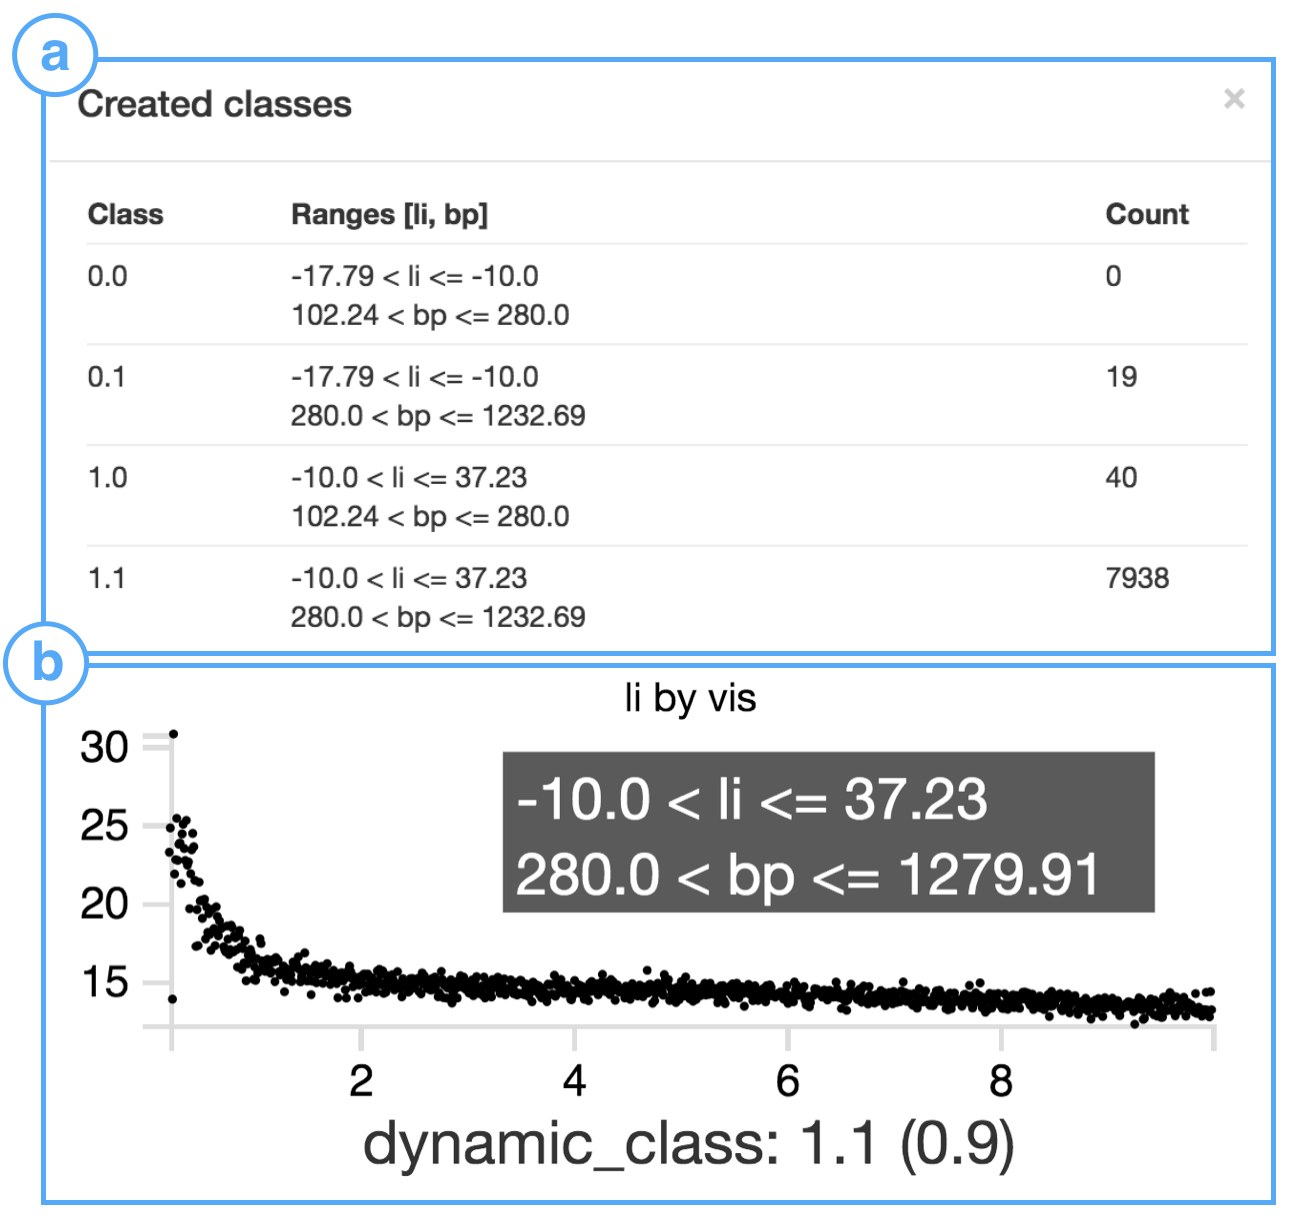
\includegraphics[width=0.7\linewidth]{figures/dcc_example.png}
\vspace{-6pt}
\caption{\tvcg{Example of dynamic classes. (a) Four different classes with different Lithium solvation energies (li) and boiling point (bp) attributes based on user-defined data ranges. (b) Users can hover over the visualizations for each dynamic class to see the corresponding attribute ranges for each class. The visualizations of dynamic classes are aggregate across all the visualizations that lie in that class based on the user-selected aggregation method.}}
\label{dcc}
\end{figure}
%%%%%%%%%%%%%%%%%%%%%%%%%%%%%%%%%
\subsection{Finer System-level Control and  Understanding}
\par During the participatory design exercise, we found that many of the features suggested by the participants indicated they wanted finer control of the system. Prior work in direct manipulation visual interfaces has suggested that finer-grained control enabled users to discover patterns and rapidly generate hypothesis based on visual feedback \cite{Shneiderman1994,Shneiderman2007a}. 
\paragraph{Controlling what the VQS does internally (all)}
In addition to query and dataset specifications, users also wanted the ability to modify the model parameters in \zv. Our findings echoed Chuang et al.~\cite{Chuang2012}, which showed that the ability to modify the model can facilitate interpretation and trust in model-driven visualizations, especially during early-stage exploration. These model parameter options include the ability to change the choice of similarity metrics (Figure \ref{zvOverview}f), the cluster size in the representative patterns (Figure \ref{zvOverview}g), setting a minimum similarity threshold for displaying the search results (Figure \ref{zvOverview}h), and the ability to tune the smoothing algorithm and parameter (Figure \ref{zvOverview}i).
\paragraph{Displaying interpretable outputs explaining how VQS arrived at recommended visualizations (all)} 
Explanatory system outputs include displaying similarity scores of the outputs, the number of datapoints in each cluster, and overlaying the original query sketch on the return visualization for comparison. We further provided display-related options for plotting modifications, including displaying error bars, and toggling between a scatterplot and line chart view.
%\cut{, and reversing the y-axis.} 
%%%%%%%%%%%%%%%%%%%%%%%%%%%%%%%%%%%%%%%%%%%%%%%%%%%%%%%%%%%%%%%%%%%%%%%%%%%%%%%%%%%%%%%%%%%%%%%%%%%%%
%!TEX root = main.tex
\section{Discussion\label{sec:guidelines}}
% In this section, we first describe a model to help characterize the design space for VQS based on the analytical workload and usage patterns from different use cases. Then, we present design challenges related to each of the process.
\subsection{Characterizing Design Space for VQSs}
Visual querying often consists of searching for a desired visualization instance across a visualization collection (Z) for a fixed visualization axes (X,Y). To characterize the design space of VQS, we introduce two axes depicting the amount of information known about visualized attribute and pattern instance, as shown in Figure~\ref{2dmodel}.
\begin{figure}[h!]
  \centering
  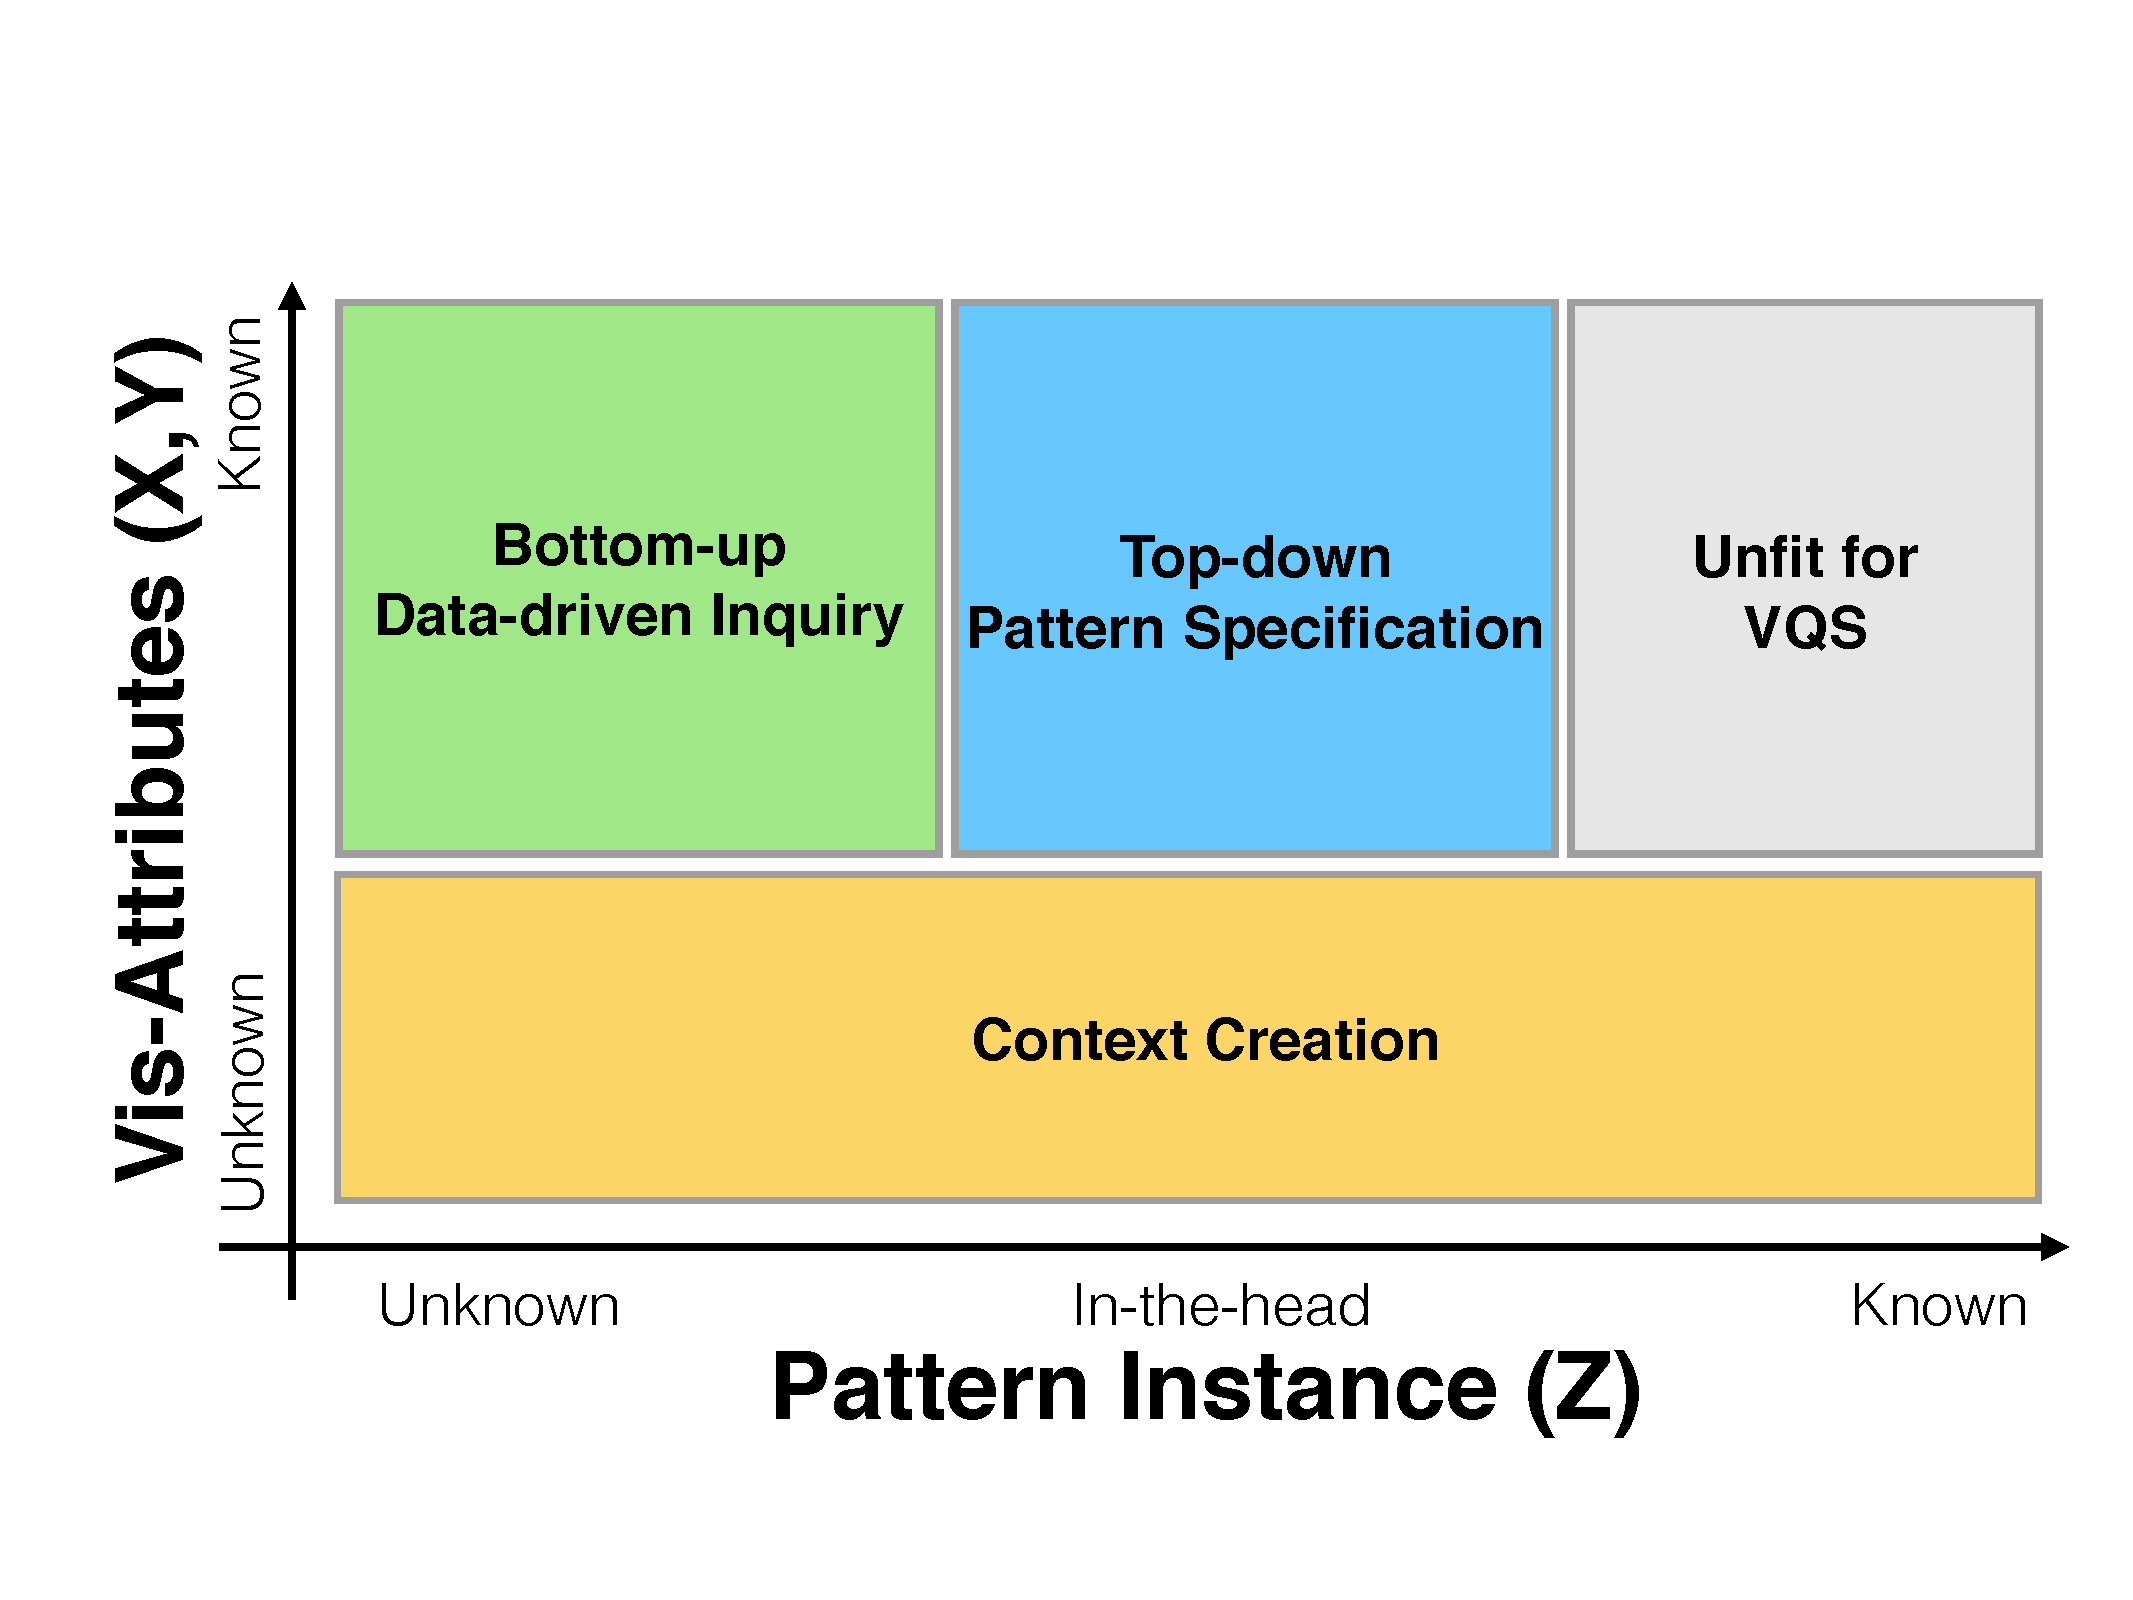
\includegraphics[width=\linewidth]{figures/2dmodel.pdf}
  \caption{The design space of VQSs is characterized by how much the analyst knows about the visualized attributes and pattern instance. Colored areas highlights the three different paradigms of VQSs. While prior work has narrowed the focus of VQSs for use cases solely in the blue region, we envision opportunities for VQSs beyond this to a larger space of use cases and problems covered also by the red and green regions.}
  \label{2dmodel}
\end{figure}
\par Along the \textbf{pattern instance} axis, the visualization instance may already be \texttt{known} to the analyst, exist as a pattern \texttt{in-the-head} of the analyst, or completely \texttt{unknown} to the analyst. For example, if a user wants to study only the pattern related to a specific gene, then the use cases is more suited for a visualization-at-a-time system, since the analyst can directly work with the visualization instance without the need for performing visual querying (Figure~\ref{2dmodel} grey). Inspired by Pirolli and Card's information foraging framework~\cite{Pirolli}, which distinguishes between information processing tasks that are \textit{top-down} (from theory to data) and \textit{bottom-up} (from data to theory), we define this search-oriented paradigm as ``top-down pattern specification'' (Figure~\ref{2dmodel} blue). On the other hand, in the realm of ``bottom-up data-driven inquiry'' (Figure~\ref{2dmodel} red), analysts often do not start with a known pattern instance. The pattern of interest is unbeknownst and external to the user and must be driven by recommendations or queries that originate from the data (or equivalently, the visualization). As we will discuss latter, this process is a crucial but understudied topic in past works on VQSs.
\par The second axis, \textbf{visualized attributes}, depicts how much the analyst knows about which X and Y axes she is interested in visualizing. Both the astronomy and genetics use cases, as well as past work in this space, had data in the form of a time series with \texttt{known} visualized attributes. In the case of our material science participants, they wanted to explore relationships between different X and Y variables. In the realm of \texttt{unknown} attributes, context creation (Figure~\ref{2dmodel} green) is essential for allowing users to pivot across different visualization subspaces. %Most past VQSs assume that the analyst has a desired pattern in-the-head that could be conveyed through visual specification, such as a sketch. 
\subsection{Design Goals and Challenges for VQS Paradigms}
In this section, we further explore the design objectives and challegnes of each paradigm. We develop a taxonomy for organizing how various features in \zv fits into the key components and paradigms as shown in Figure~\ref{fig:taxonomy}.
\begin{figure*}[ht!]
  \centering
  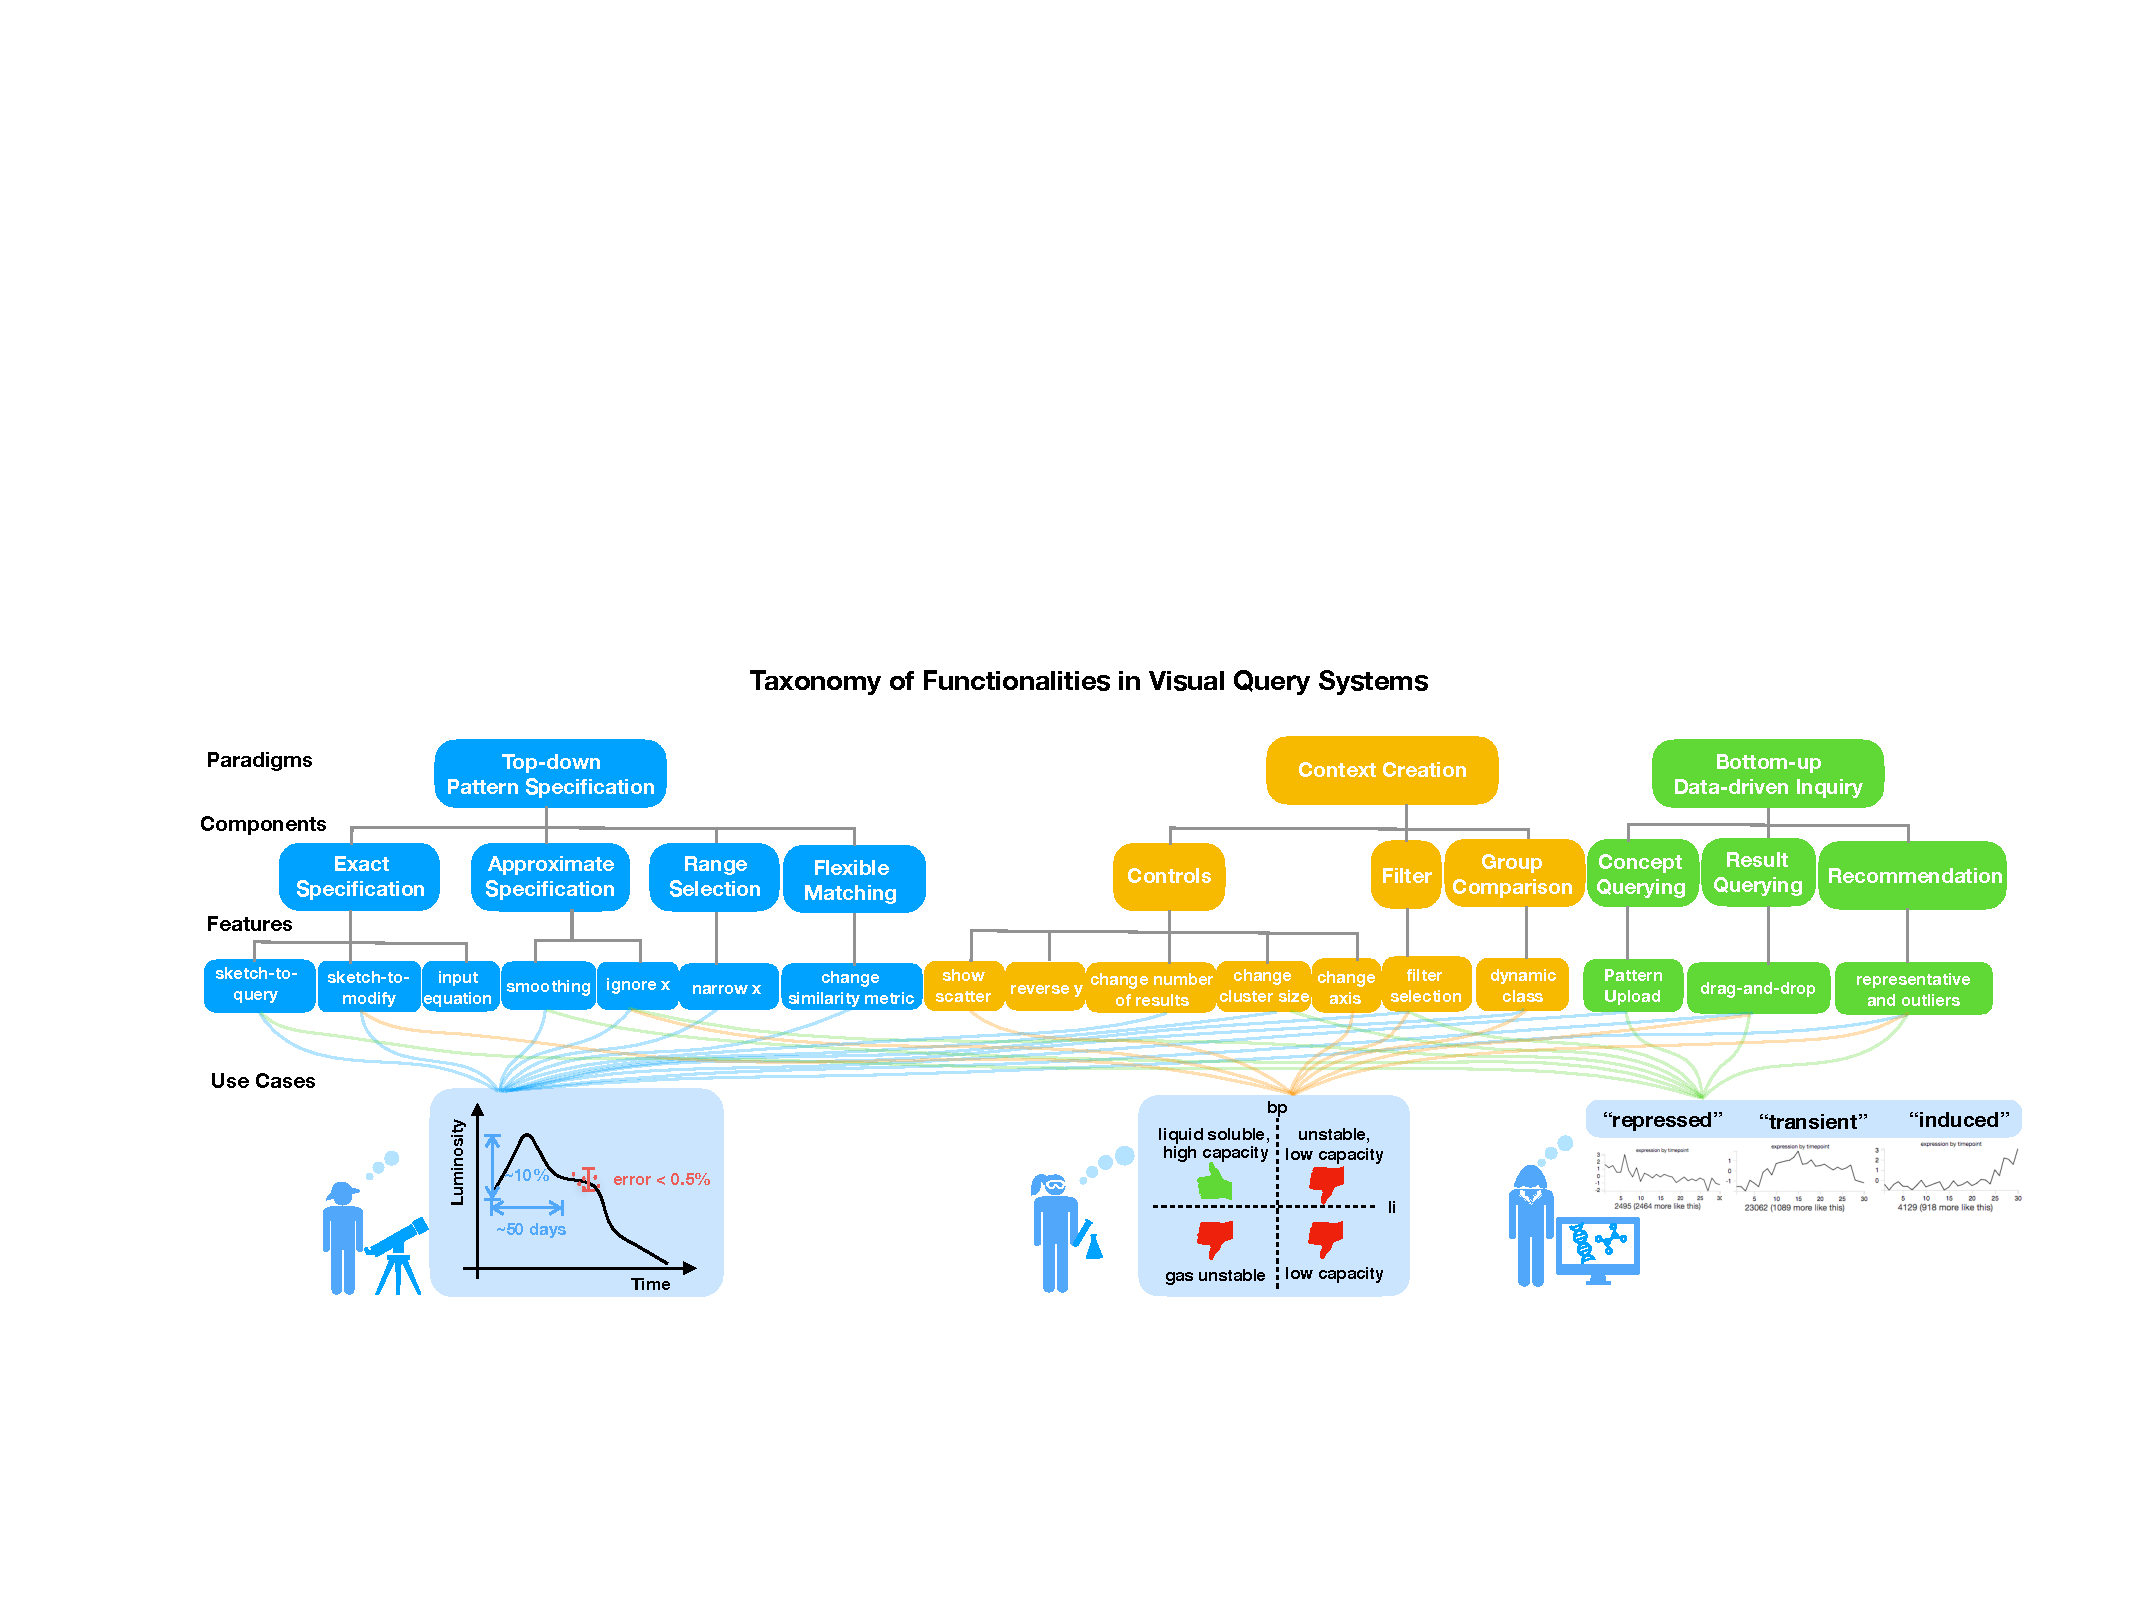
\includegraphics[width=\linewidth]{figures/full_taxonomy.pdf}
  \caption{Taxonomy of functionalities in VQSs. From top, each of the three paradigm is broken down into key components in the system, which is instantiated as features in \zv. The bottom-most layer connects the use cases features that have practical or envisioned usage based on the evaluation study.}
  \label{fig:taxonomy}
\end{figure*}
% \par Drawing from our participatory design experience, evaluation study, and literature review in this space, we design a taxonomy for understanding the key functionalities in VQSs. In Figure~\ref{fig:taxonomy}, we show how each use cases makes use of the different features in \zv, then we organize the features into key components for VQSs, which belongs to one of the three paradigms in the VQS design space. 
In particular, we will describe the main form of inquiry addressed by each paradigm (\textit{what, where, which}), the characteristic use case, and design challenges involved in building features that support these paradigms.
\boldpara{Top-down Pattern Specification:} Top-down approaches starts with user's intuition about how their desired patterns should look like based on `theory', including visualizations from past experiences or an abstract conceptions based on external knowledge. The goal of top-down pattern specification is to address the \textit{which} questions in visual sensemaking (\textit{which pattern instance exhibits this pattern?}), effectively moving rightwards to the gray area in Figure~\ref{2dmodel} where the pattern instance is known. 
\par Based on this preconceived notion of what to search for, the design challenge is to translate the query in the analyst's head to a query executable by the VQS. As shown in Figure~\ref{fig:taxonomy}, this includes both components for specifying the pattern as well as controls governing the underlying algorithm of how the shape-matching is performed. For example, A1 knows intuitively what a supernovae pattern looks like and the detailed constraints on the shape, such as the width and height of the peak as well as the level of signal-to-noise tolerance for defining a match. He performs exact specification through sketching, choses the option to ignore differences on the x axis, and changes the similarity metric for flexible matching.  %The design challenge of top-down pattern specification is to ----- enable users to How to translate the in-the-head query to visual query and how matching is done. 
\boldpara{Bottom-up data-driven inquiry:} While the usage of each querying feature may vary from one participant to the next, generally, result querying and pattern upload are considered bottom-up approaches that go from data to theory by enabling users to query via examples of known visualizations. Bottom-up data-driven inquiries addresses the \textit{what} questions in the sensemaking process. For example, genetics participants do not have a preconceived knowledge of what to search for in the dataset. They were mostly interested in \textit{what types of patterns exist in the dataset} through representative trends and therefore queried mainly through these recommended results to jumpstart further queries. The goal of data-driven inquiry is to move towards the blue area in Figure~\ref{2dmodel}where the analyst gains some in-the-head notion of what the pattern looks like. The design challenge of bottom-up approaches includes designing the right set of `stimuli' that could provoke further data-driven inquiries, as well as low-effort mechanisms to search via these results.
\boldpara{Context Creation:} Analysts often navigate across different parts of the visualization subspace to narrow to a more manageable scope or to explore relationships between different visualization attributes. Context creation addresses the \textit{where} question of sensemaking by enabling analyst to pivot across different visualization collections. The goal is to learn about \textit{where are the patterns of interest?}, effectively moving upwards in Figure~\ref{2dmodel} along the known attributes region. For example, material scientists often do not start with a pattern in-the-head, but recognize salient trends such as inverse correlation or linear correlation. They switch between different visualized attributes or create different dynamic classes to study their data from different perspectives. The design challenge of context creation is to develop features that serve as `lenses' to navigate users to desired regions of the data, visualize and compare how the data changes between different contexts and ensure that the context is dynamically reflected across other functionalities in the VQSs.
\begin{figure}[h!]
  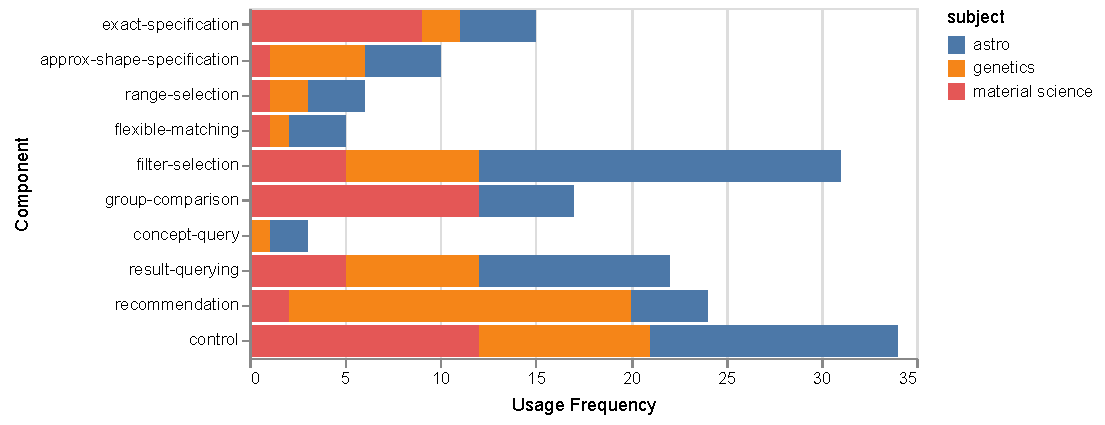
\includegraphics[width=\linewidth]{figures/usagefreqbysubject.pdf}
  \caption{The number of times each component is used during the evaluation study, broken down by subject areas. Astronomers largely focused on filtering, whereas material scientists made heavy use of dynamic class and geneticists made use of recommendations heavily.}\label{fig:usagefreqbysubject}
\end{figure}
\par The three paradigm that we have described are not mutually exclusive categories. In fact, we find that participants often construct a central workflow focussed on features from one of the main paradigms and interleave variations with the feature usage from the two other paradigms as they iterate on the analytic task, as shown in Figure~\ref{fig:usagefreqbysubject}. As we have seen, the central paradigm adopted by each use case is tightly coupled with characteristics of the analytic challenges presented by the use cases. Next, we will describe some of the design principles (DP) based on our study findings.
% \par As illustrated in Figure \ref{fig:sbmodel}, our search-browse paradigm is motivated by the characteristic challenges and foraging acts each use cases pose on existing VQSs observed in our design study. 
% \par In the astronomy use case, the participants knew the patterns they are looking for, but the patterns are hard to specify and find. The main challenge for the VQS involves finer specification of sketched patterns, such as amplitude and width of the peak and noise level tolerance for defining a pattern match. Describe more in D1. The main workflow for the astronomers in our user study involves \textit{enriching}, either through finer query specification or via filtering data subsets, to increase the probability that their queries would be more accurately matched with what they are looking for.

% %For example, G2 knew that there was three repeated measurements that was taken for every timestep, in one of the profiles there was a sharp jump whereas other datapoints are relatively flat, he then concludes by inspecting in the scatterplot view that the rise in gene expression is probably due to an experimental error rather than the activation of a gene, because the other two repeated measurements were similar in magnitude. In other words, the scatterplot view offered him density of points as another proxy to consider that was not offered in the line chart perspective.
%  %This is true for both participants with and without a desired pattern in mind. For the participant without a desired pattern (G2), he created groups based on quartile statistics of additional data attributes and recorded the most significant representative pattern.

% - What does the act of browsing and searching mean in the context of VQSs
%   - browse: viewing ranked result and any recommended results on the side, derived from the data and analysis context.
%   - search: act of going from a user's in-the-head concept to an actionable query that could be executed through the VQSs, most work have focussed on sketch, we allow more than this.
%   - The challenge of browsing and searching is well-known in information retrieval~\cite{Olston2003}, browse alone is limited by how much a user can browse and process at once, search alone can be ambiguous without sufficient context from looking at example results.
% \par Pirolli and Card's notional model further characterizes the trade-offs between three central activities in the information foraging process: exploring, enriching, and exploiting~\cite{Pirolli}.  We organize the features that we have developed in \zv into these foraging acts, as shown in Figure~\ref{feature_heatmap}.
% \par We find that participants often create unexpected workflows that chain together multiple analysis steps, including interactions, controls, and queries in order to address a higher-level research question. We find that participants often construct a central workflow, \tvcg{which they then iterate on while adding additional variations.} Their \emph{central workflow often resembles one of the three foraging acts} that aligns with the type of research question and dataset they are interested in. The variations are based on intermixing their central workflow with the other two foraging \tvcg{acts}.
% % We find that participants often have a strong inclination to perform tasks that resembles one of the three foraging act and sparsely intermixed with other activities to support their analysis, depending on the type of research question and dataset they are interested in.
% \par As illustrated in Figure \ref{fig:sbmodel}, our search-browse paradigm is motivated by the characteristic challenges and foraging acts each use cases pose on existing VQSs observed in our design study. For example, the genetics participants do not have a preconceived knowledge of what they want to search for in the dataset. They were mostly interested in \textit{exploring} clusters to gain an overall sense what profiles exist in the dataset \tvcg{through representative trends} and therefore queried mainly through drag-and-drop to jumpstart further queries. Point to need for D3 and D4. The variations to their main workflow include changing cluster sizes and display settings to offer them different perspectives on the dataset (\textit{exploit}) and filtering on data attributes (\textit{enriching}).
% \par In the astronomy use case, the participants knew the patterns they are looking for, but the patterns are hard to specify and find. The main challenge for the VQS involves finer specification of sketched patterns, such as amplitude and width of the peak and noise level tolerance for defining a pattern match. Describe more in D1. The main workflow for the astronomers in our user study involves \textit{enriching}, either through finer query specification or via filtering data subsets, to increase the probability that their queries would be more accurately matched with what they are looking for.
% \par The main workflow for material scientists involves \textit{exploiting}, since they spend the majority of their efforts performing ``close-reading'' of individual visualizations to understand the relationships between physical variables. The participants are able to identify interesting relationships between physical variables when they examine each closely, but they are not sure what patterns to look for to begin with. More in D2.
% %For example, G2 knew that there was three repeated measurements that was taken for every timestep, in one of the profiles there was a sharp jump whereas other datapoints are relatively flat, he then concludes by inspecting in the scatterplot view that the rise in gene expression is probably due to an experimental error rather than the activation of a gene, because the other two repeated measurements were similar in magnitude. In other words, the scatterplot view offered him density of points as another proxy to consider that was not offered in the line chart perspective.
%  %This is true for both participants with and without a desired pattern in mind. For the participant without a desired pattern (G2), he created groups based on quartile statistics of additional data attributes and recorded the most significant representative pattern.
% % [---] out of 9 of our participants had more than one main workflow.

\subsection{DP1: The Inefficiency of Sketch}
% \subsection{DC3: Closing the loop in VQS sense-making cycle with bottom-up data-driven inquries}
\par Our interactions with the scientists showed that different modalities for inputting a query can be useful for different problem contexts. To our surprise, despite the prevalence of sketch-to-query systems in literature, only two out of our nine users had a practical usage for querying by sketching. %Overall, bottom-up querying via drag-and-drop was more intuitive and more commonly used than top-down querying methods, such as sketching or input equations.
\par The main reason why participants did not find sketching useful was that they often do not start their analysis with a pattern in mind. Later, their intuition about what to query is derived from other visualizations that they see in the VQS, in which case it made more sense to query using those visualizations as examples directly. In addition, even if a user has a query pattern in mind, sketch queries can be ambiguous or even impossible to draw by sketching (e.g. A2 looked for a highly-varying signal enveloped by a sinusoidal pattern indicating planetary rotation 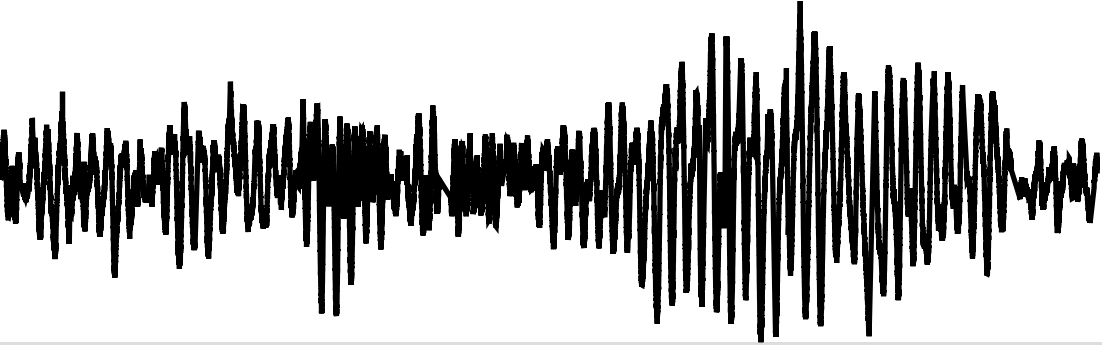
\includegraphics[width=1.55\baselineskip,keepaspectratio]{figures/impossible_sketch.png}).
\par The latter case is also supported by the unexpected use cases where sketching was simply used as a mechanism to modify dragged-and-dropped queries. As shown in Figure \ref{query_modification} (top), M2 first sketched a pattern to find solvent classes with anticorrelated properties. However, the sketched query did not return visualizations of interest. So, he instead dragged and dropped one of the peripheral visualizations that was close enough to his desired visualization to the sketchpad and then smoothed out the noise due to outlier datapoints by tracing a sketch over the visualization. M2 repeated this workflow twice in separate occurrences during the study and was able to derive insights from the results. Likewise, A3 was interested in pulsating stars characterized by dramatic changes in the amplitudes of the light curves. During the search, hotspots on stellar surfaces often show up as false positives as they also result in dramatic amplitude fluctuations, but happen at a regular intervals. In the VQS, A3 looked for patterns that exhibits amplitude variations, but also some irregularities. As shown in Figure \ref{query_modification} (bottom), she first picked out a regular pattern (suspected star spot), then modified it slightly so that the pattern looks more irregular.
\begin{figure}[ht!]
    \centering
    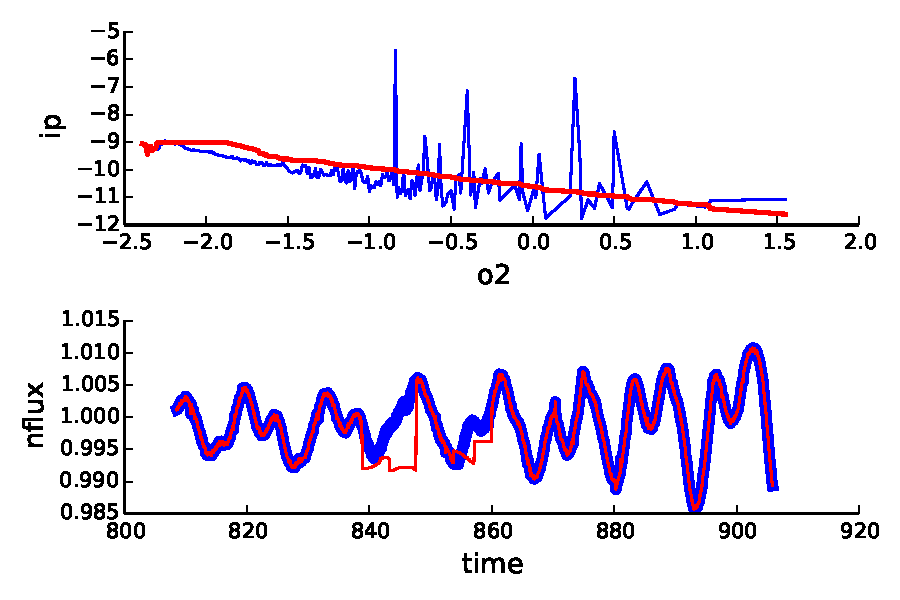
\includegraphics[width=\columnwidth]{figures/QueryModificationBySketch.pdf}
    \caption{\tvcg{Examples of query modification by M2 (top) and A3 (bottom) performed during the study The inital drag-and-dropped query is shown in blue and the sketch-modified queries in red.}
    \label{query_modification}}
    \vspace{-10pt}
\end{figure}
\par The lack of practical use of top-down pattern specification is also reflected in the fact that querying by equation is unpopular. Both querying mechanism adopt a problematic assumption that analysts start with a known and easy-to-specify search pattern in mind. In both astronomy and genetics use cases, the visualization patterns result from complex physical processes that could not be written down as an equation analytically. Even in the case of material science when analytical relationships do exist, it is challenging to formulate functional forms in an prescriptive, ad-hoc manner.
% Despite functional fitting being common in scientific data analysis, Figure \ref{feature_heatmap} shows that
% . However, 
\par Both of these findings suggest that while sketching is an useful analogy for people to express their queries, \emph{the existing ad-hoc, sketch-only model for visualization querying is insufficient without data examples that can help analysts jumpstart their exploration}. Table~\ref{table:relatedwork} show that most past work focus on optimizing the components in the top-down paradigm, missing out largely on the key components in the other two paradigms, indicated by the absence of green features on the right hand side of the table. We suspect that the limited coverage in addressing different types of analytics use cases may be why existing sketch-to-query systems are not commonly adopted in practice. %This result points to a need for ----- in future VQSs. %This, however, points to an exciting direction for sketching interface in VQSs for developing advanced drawing and modification tools that enable more precise visualization query specification.}
%For instance, material science discovered a known inverse relationship during exploration
%Which is really interesting. Which is something that we observed experimentally also. That is an interesting insight right htere. This seems to suggest that there is a fundamental issue in if you want to try to get better on this axis, and get as low as possible, you lose out on the other axis.
%once they see it they know it but they don't know beforehand

\subsection{DP2: Practical Use of Bottom-up approaches}
\par Our results indicate that \emph{bottom-up data-driven inquiries are more common than top-down pattern specification when the users have no desired patterns in mind}, which is commonly the case for exploratory data analysis. Examples of practical uses of result querying includes inspecting the top-most similar visualizations that lie in a cluster and finding visualizations that are similar to an object of interest that exhibits a desired pattern. 
\par Likewise, many participants envisioned use cases for pattern loading. The ability to load in data patterns as a query would enable users to compare visualizations between different experiments, species, or surveys, query with known patterns from an external reference catalog (e.g. important genes of interest, objects labeled as supernovae), or verify the results of a simulation or downstream analysis by finding similar patterns in their existing dataset. Users can also specify a more precise query that captures the essential shape features of a desired pattern (e.g. amplitude, width of peak), that cannot be precisely sketched. For example, the width of a supernovae light curve is characteristic to the radioactive decay rate of its chemical signature~\cite{Nugent1997}, so querying with an exact pattern template would be helpful for distinguishing the patterns of interest from noise.
\par The prevalence of bottom-up approaches not only point to the need for supporting result querying in VQSs, but also to the need for providing recommendation for users who may not have a desired pattern in mind. We found that geneticists often gain their intuition about the data from the recommended representative trends. One example of rapid insight discovery comes from G2 and G3, who identified that the three representative patterns shown in \zv---induced genes (profiles with expression levels staying up), repressed genes (started high but went down), and transients (go up and then come down at different time points)---corresponded to the same three groups of genes discussed in a recent publication\cite{Gloss2017}. The clusters provoked G2 to generate a hypothesis regarding the properties of transients: \textit{``Is that because all the transient groups get clustered together, can I get sharp patterns that rise and ebb at different time points?''} To verify this hypothesis, G2 increased the parameter controlling the number of clusters and noticed that the cluster no longer exhibited the clean, intuitive patterns he had seen earlier. G3 expressed a similar sentiment and proceeded by inspecting the visualizations in the cluster via drag-and-drop. He found a group of genes that all transitioned at the same timestep, while others transitioned at different timesteps. G3 described the process of using VQSs as doing ``detective work'' that provoked him to generate further scientific hypotheses as well as data actions.
\par By browsing through the ranked list of result, representative, and outlier in \zv, participants were also able to gain a peripheral overview of the data and spot anomalies during exploration. For example, A1 spotted time series that were too faint to look like stars after applying a filter constraint of CLASS\_STAR=1. After a series of query results browsing and consultation with an external database, he concluded that the dataset had been incorrectly labelled with all the stars with CLASS\_STAR=0 as 1 during data cleaning. These examples show that both the browsing-act through recommendations and performing search via these results are essential for `closing the loop' between the sensemaking acts in VQSs. 
\subsection{DP3: Enriching Search with Context}
\par Past studies in taxonomies of visualization tasks have shown that it is important to design features that enable users to select relevant subsets of data in visual analytics\cite{Amar2005,Heer2012}. %We designed two dynamic faceting features coupled with coordinated views that enabled users to specify subsets of data they are querying on and see immediate changes updated in the query, representative, and outlier results.
We found that all participants either envisioned a use case or utilized components of the context creation paradigm offered in \zv to explore and compare subsets of their data.
\par A1 expressed that even though the filtering step could be easily done programmatically on the dataset and reloaded into \zv, filtering on-the-fly was a powerful way to dynamically test his hypothesis. Interactive filtering lowers the barrier between the iterative hypothesize-then-compare cycle, thereby enabling participants to test conditions and tune values that they would not have otherwise modified.
% echoing our previous finding that segmented workflow prevents extensive exploration.
During the study, participants used filtering to address questions such as: \textit{Are there more genes similar to a known activator when we subselect only the differentially expressed genes?} \texttt{DIFFEXP=1} (G2) or \textit{Can I find more supernovae candidates if I query only on objects that are bright and classified as a star?} \texttt{flux\textgreater10 AND CLASS\_STAR=1} (A1). Three participants had also used filtering as a way to pick out individual objects of interest to query with. For example, G2 set the filter as gene=9687 and explained that since ``this gene is regulated by the estrogen receptor, when we search for other genes that resemble this gene, we can find other genes that are potentially affected by the same factors.''
\par While filtering enabled users to narrow down to a selected data subset, dynamic class creation enabled users to compare relationships between multiple attributes and between subgroups of data. For example, M2 divided solvents in the database to eight different categories based on voltage properties, state of matter, and viscosity levels, by dynamically setting the cutoff values on the quantitative variables to create these classes. By exploring these custom classes, M2 learned that the relationship between viscosity and lithium solvation energy is independent of whether a solvent belongs to the class of high voltage or low voltage solvents and cited that dynamic class creation was central to learning about this previously-unknown attribute properties:
\begin{quote}
All this is really possible because of dynamic class creation, so this allows you to bucket your intuition and put that together. [...] I can now bucket things as high voltage stable, liquid stable, viscous, or not viscous and start doing this classification quickly and start to explore trends. [...] And look how quickly we can do it! Quite good!
\end{quote}
Context creation enables users to change the lens in which they look through when preforming visual querying, thereby creating more opportunities to see the queried data from different perspectives.
%Context creation is a useful ---- despite the --- pattern instance. Filtering still useful 
%\par Participants employed \emph{a mix of bottom-up and top-down approaches when faceting through data in VQS}, including narrowing the search space based on some intuition about a phenomena, selecting individual visualizations, or specifying high-level groupings to compare and query with.
%!TEX root = main.tex
\section{Conclusion\label{sec:conclusion}}
While VQSs hold tremendous promise in accelerating data exploration, they are rarely used in practice. In this paper, we worked closely with analysts from three diverse domains to characterize how VQSs can address their analytic challenges, collaboratively design VQS features, and evaluate how VQS functionalities are used in practice. Participants were able to use our final deployed system, \zvpp, for discovering desired patterns and trends, and obtaining valuable insights to address unanswered research questions. Grounded in these experiences, we developed a sensemaking model for how analysts make use of VQSs. Contrary to past work, we found that sketch-to-query is not as effective in practice as past work may suggest. Beyond sketching, we find that each sensemaking process fulfills a central role in participants' analysis workflows to address their high-level research objectives. We advocate that future VQSs should invest in understanding and supporting all three sensemaking processes to effectively `close the loop' in how analysts interact and perform sensemaking with VQSs. While more work certainly remains to be done, by contributing to a better understanding of how VQSs are used in practice across domains, our paper can also serve as a roadmap for broader adoption of VQSs,
and hopefully trigger exploration of novel use cases for these tools.
% the application of VQSs to ---- opportunities beyond ----
% for the broad adoption of VQSs in data analysis, opening up potential unexplored use cases and opprtunity for VQS. envision opportunities for VQSs beyond this to a larger space of use cases.
% process In discovering two ----- en ---opening up pathways  potential pathway worflow, while clo---- . 
% learn about the challenges they face when working with data. We extended our VQS \zv to the point where it could be effectively used for scientific data analysis. 
% Through participatory design, we identified three classes of missing interface capabilities  essential for employing VQSs for facilitating insight in real scientific applications, spanning expressive querying and dynamic faceting, as well as fine-grained control and understanding, along with the ability to compose flexible workflows in an integrated manner (RQ2). Finally, our evaluation study demonstrated how these features helped accelerate scientific insights (RQ3), as well as how they fit in the context of data analysis workflows (RQ4). One such finding is that bottom-up querying (e.g., drag-and-drop) is preferred over top-down (e.g., sketching) for exploratory data analysis, contrary to what is commonly supported in existing VQSs.
% point to focus on sci data but future work on quantified self and social viz
% VQS important 
% Our work : 
% - \zvpp
% - sensemaking model 
% domain problem characterization of visual querying through design studies with three different subject areas,
% \item abstraction of taxonomy and design space of VQSs grounded in participatory design findings,
% \item a full-fledge VQS, \zvpp, capable of facilitating rapid hypothesis generation and insight discovery,
% \item evaluation study findings regarding how VQSs are used in practice, leading to the formation of a novel sensemaking model for VQSs. %including the ineffectiveness of sketching and the ---- workflow  
% discover sketch 
% Our work closes the loop in VQS sensemaking so that VQS works in scenarios  where XY is unknown or Z is unknown. These areas were previously unexplored by past works.
% As presented in this section, our study is the first that contributes towards a holistic understanding of the sensemaking process for visual querying.
% ----- how they are used in practice. %Rather than assuming visual querying through sketch is useful, we 
% Our work is the first that evaluate on multiple case study participatory design, longitudinal study. 
% Participants intermixed functionalities across different sensemaking paradigms to address their problem contexts.
 % more thoroughly characterize the problem design space of VQSs and taxonomy abstraction for understanding the sensemaking process in VQSs. Moreover, we performed design studies with three different subject areas with a diverse set of questions, datasets, and challenges to further generalize our findings.
 % facilitating a diverse set of potential workflows and 
 % Both query by sketch and equations adopt a problematic assumption that analysts start with a known and easy-to-specify search pattern in mind. 
\bibliographystyle{ACM-Reference-Format}
\bibliography{reference}
\end{document}
